
\subsection{Supplementary Figures}


\clearpage
\begin{figure}
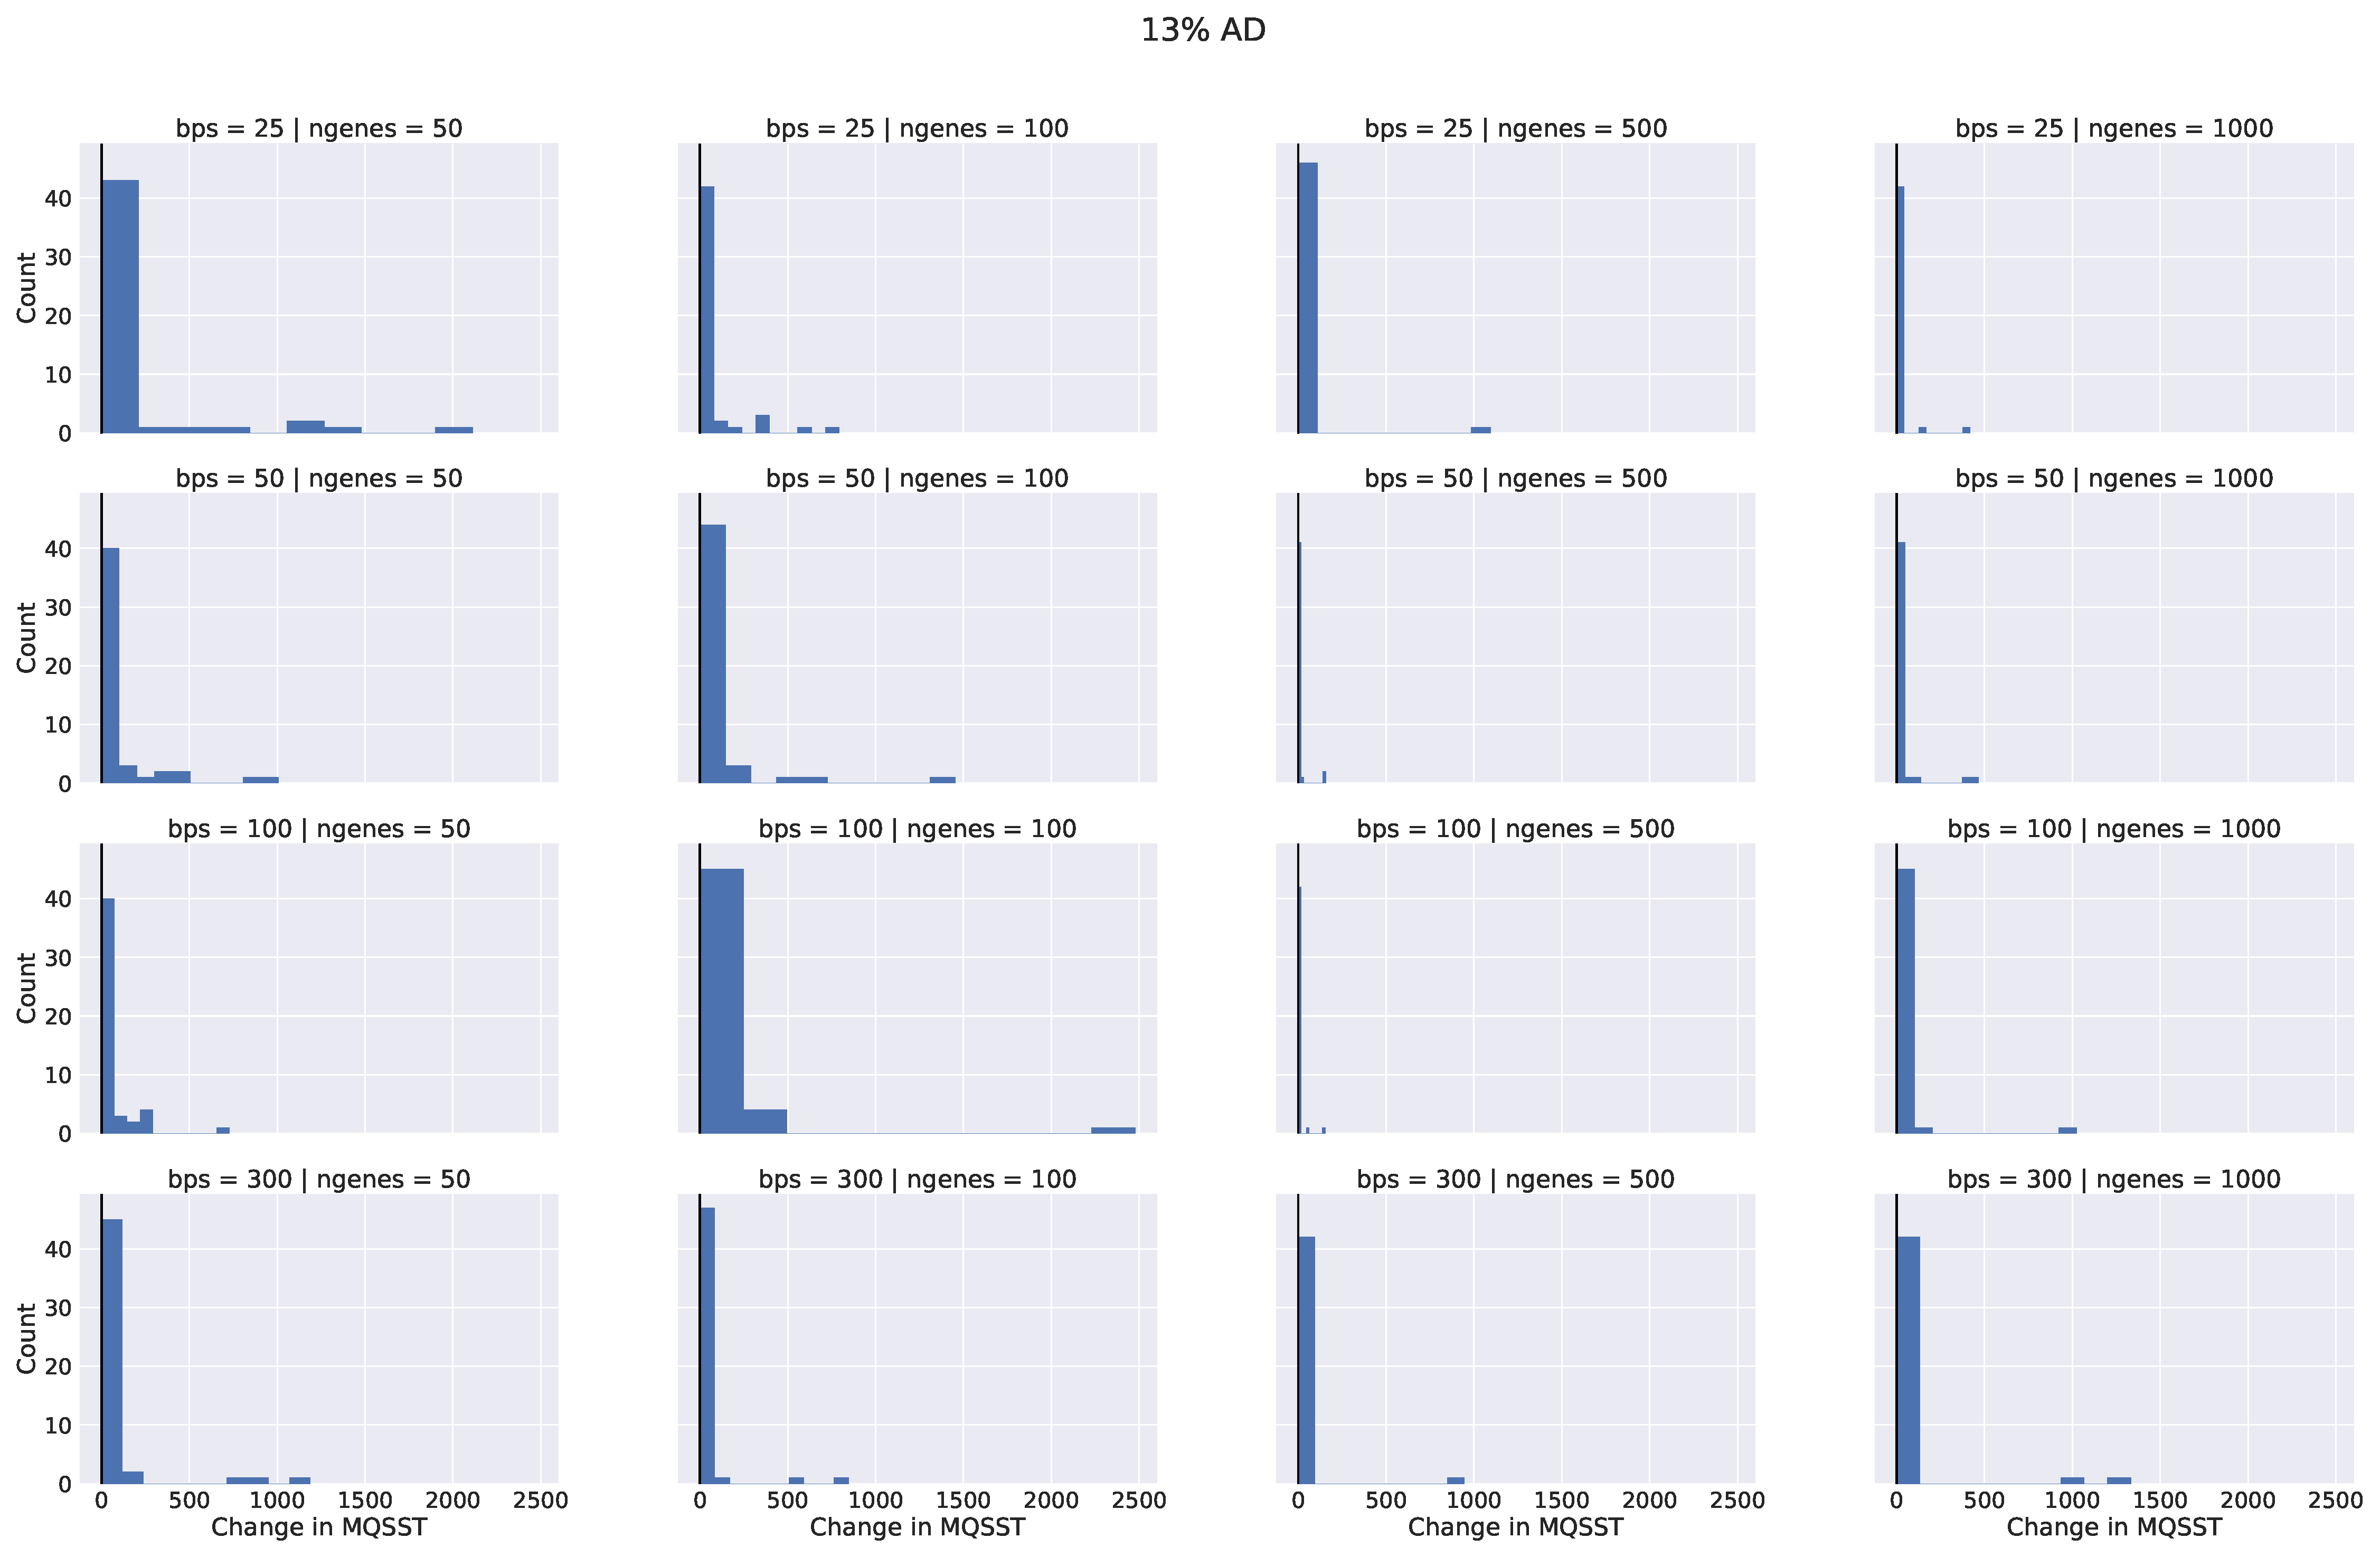
\includegraphics[width=\textwidth]{svdquest-figs/all-scorediffs-hist-cgenes-13.eps}
\caption[Histogram of differences in MQSST scores between SVDquartets+PAUP* and SVDquest* for the low ILS 50-taxon datasets]{Histogram of the difference in MQSST scores between
  SVDquartets+PAUP* and SVDquest*  on low ILS (AD = 13\%) 50-taxon c-gene data
  with 40-50 replicates per model condition (i.e. a specific combination of ILS level, number of genes, and sequence length). Positive x-values
  indicate that SVDquest* finds a larger MQSST score than
  SVDquartets+PAUP*.}
  \label{fig:s1}
\end{figure}




\clearpage

\begin{figure}
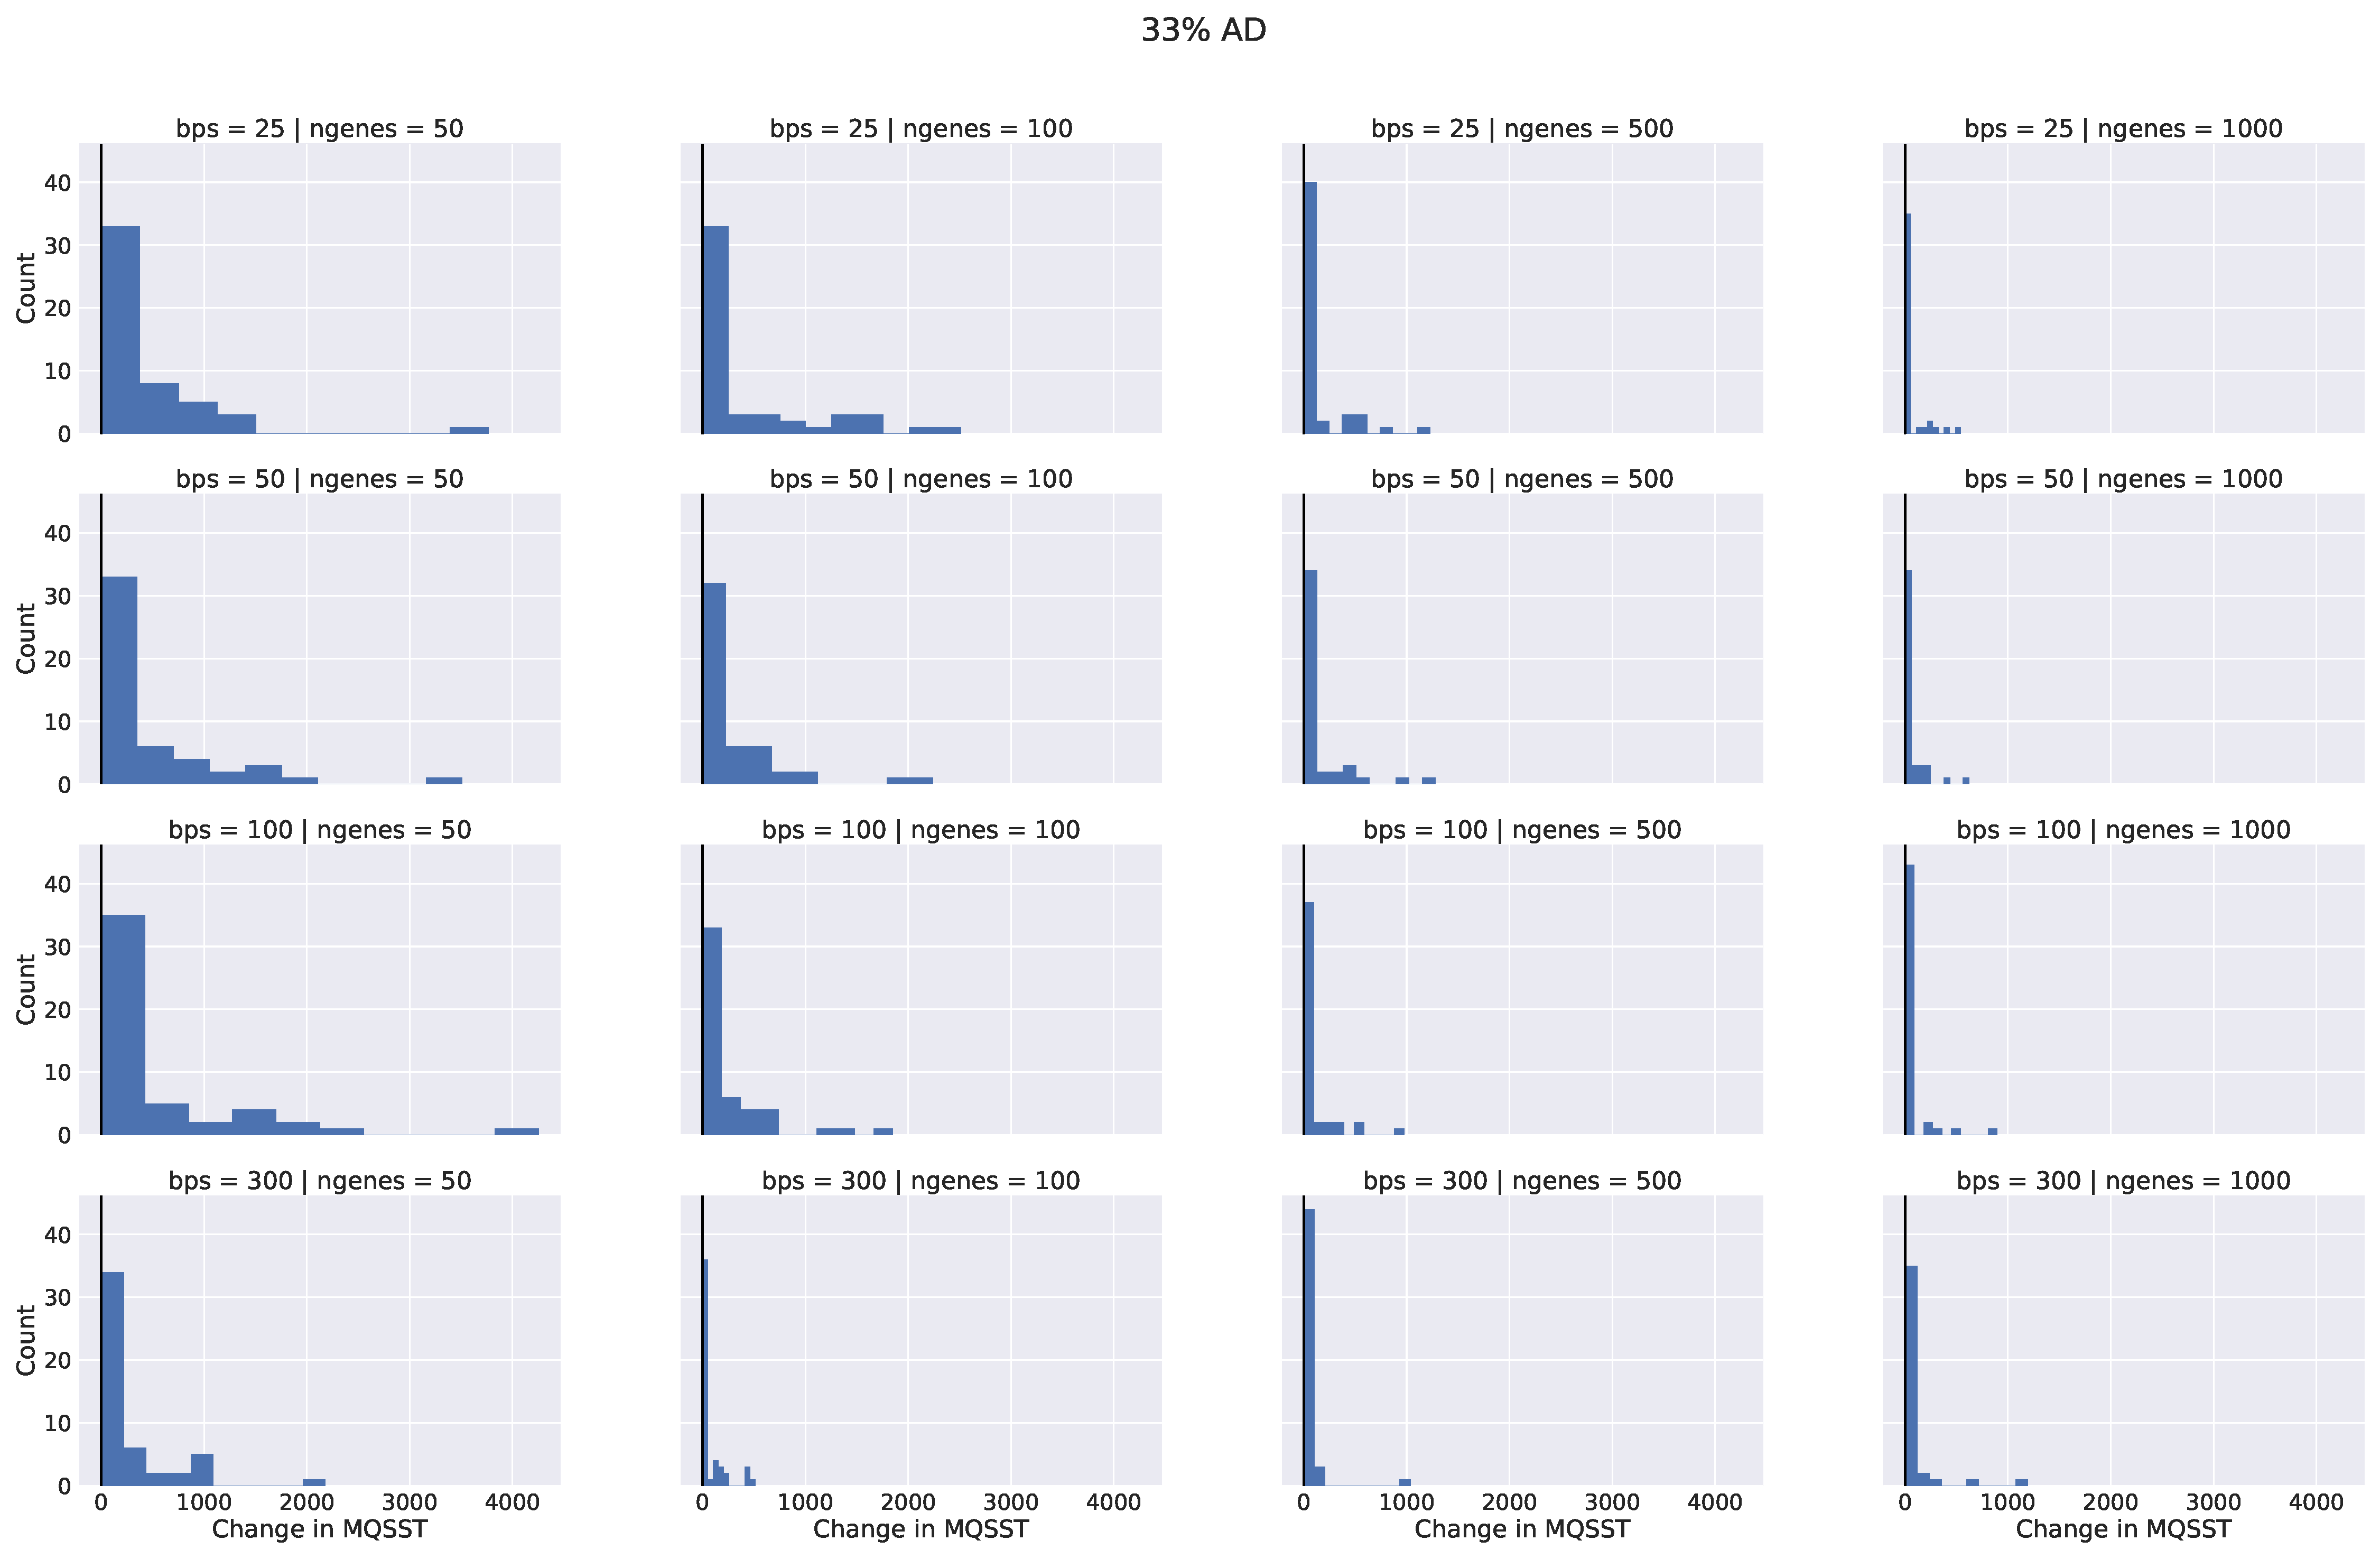
\includegraphics[width=\textwidth]{svdquest-figs/all-scorediffs-hist-cgenes-33.eps}
\caption[Histogram of differences in MQSST scores between SVDquartets+PAUP* and SVDquest*  for the high ILS 50-taxon datasets]{Histogram of the difference in MQSST scores between
  SVDquartets+PAUP* and SVDquest*   on high ILS 
  (AD = 33\%) 50-taxon c-gene data
  with 40-50 replicates per model condition (i.e. a specific combination of ILS level, number of genes, and sequence length). 
  Positive x-values
  indicate that SVDquest* finds a larger MQSST score than
  SVDquartets+PAUP*.
}
\label{fig:s2}
\end{figure}

\clearpage

\begin{figure}
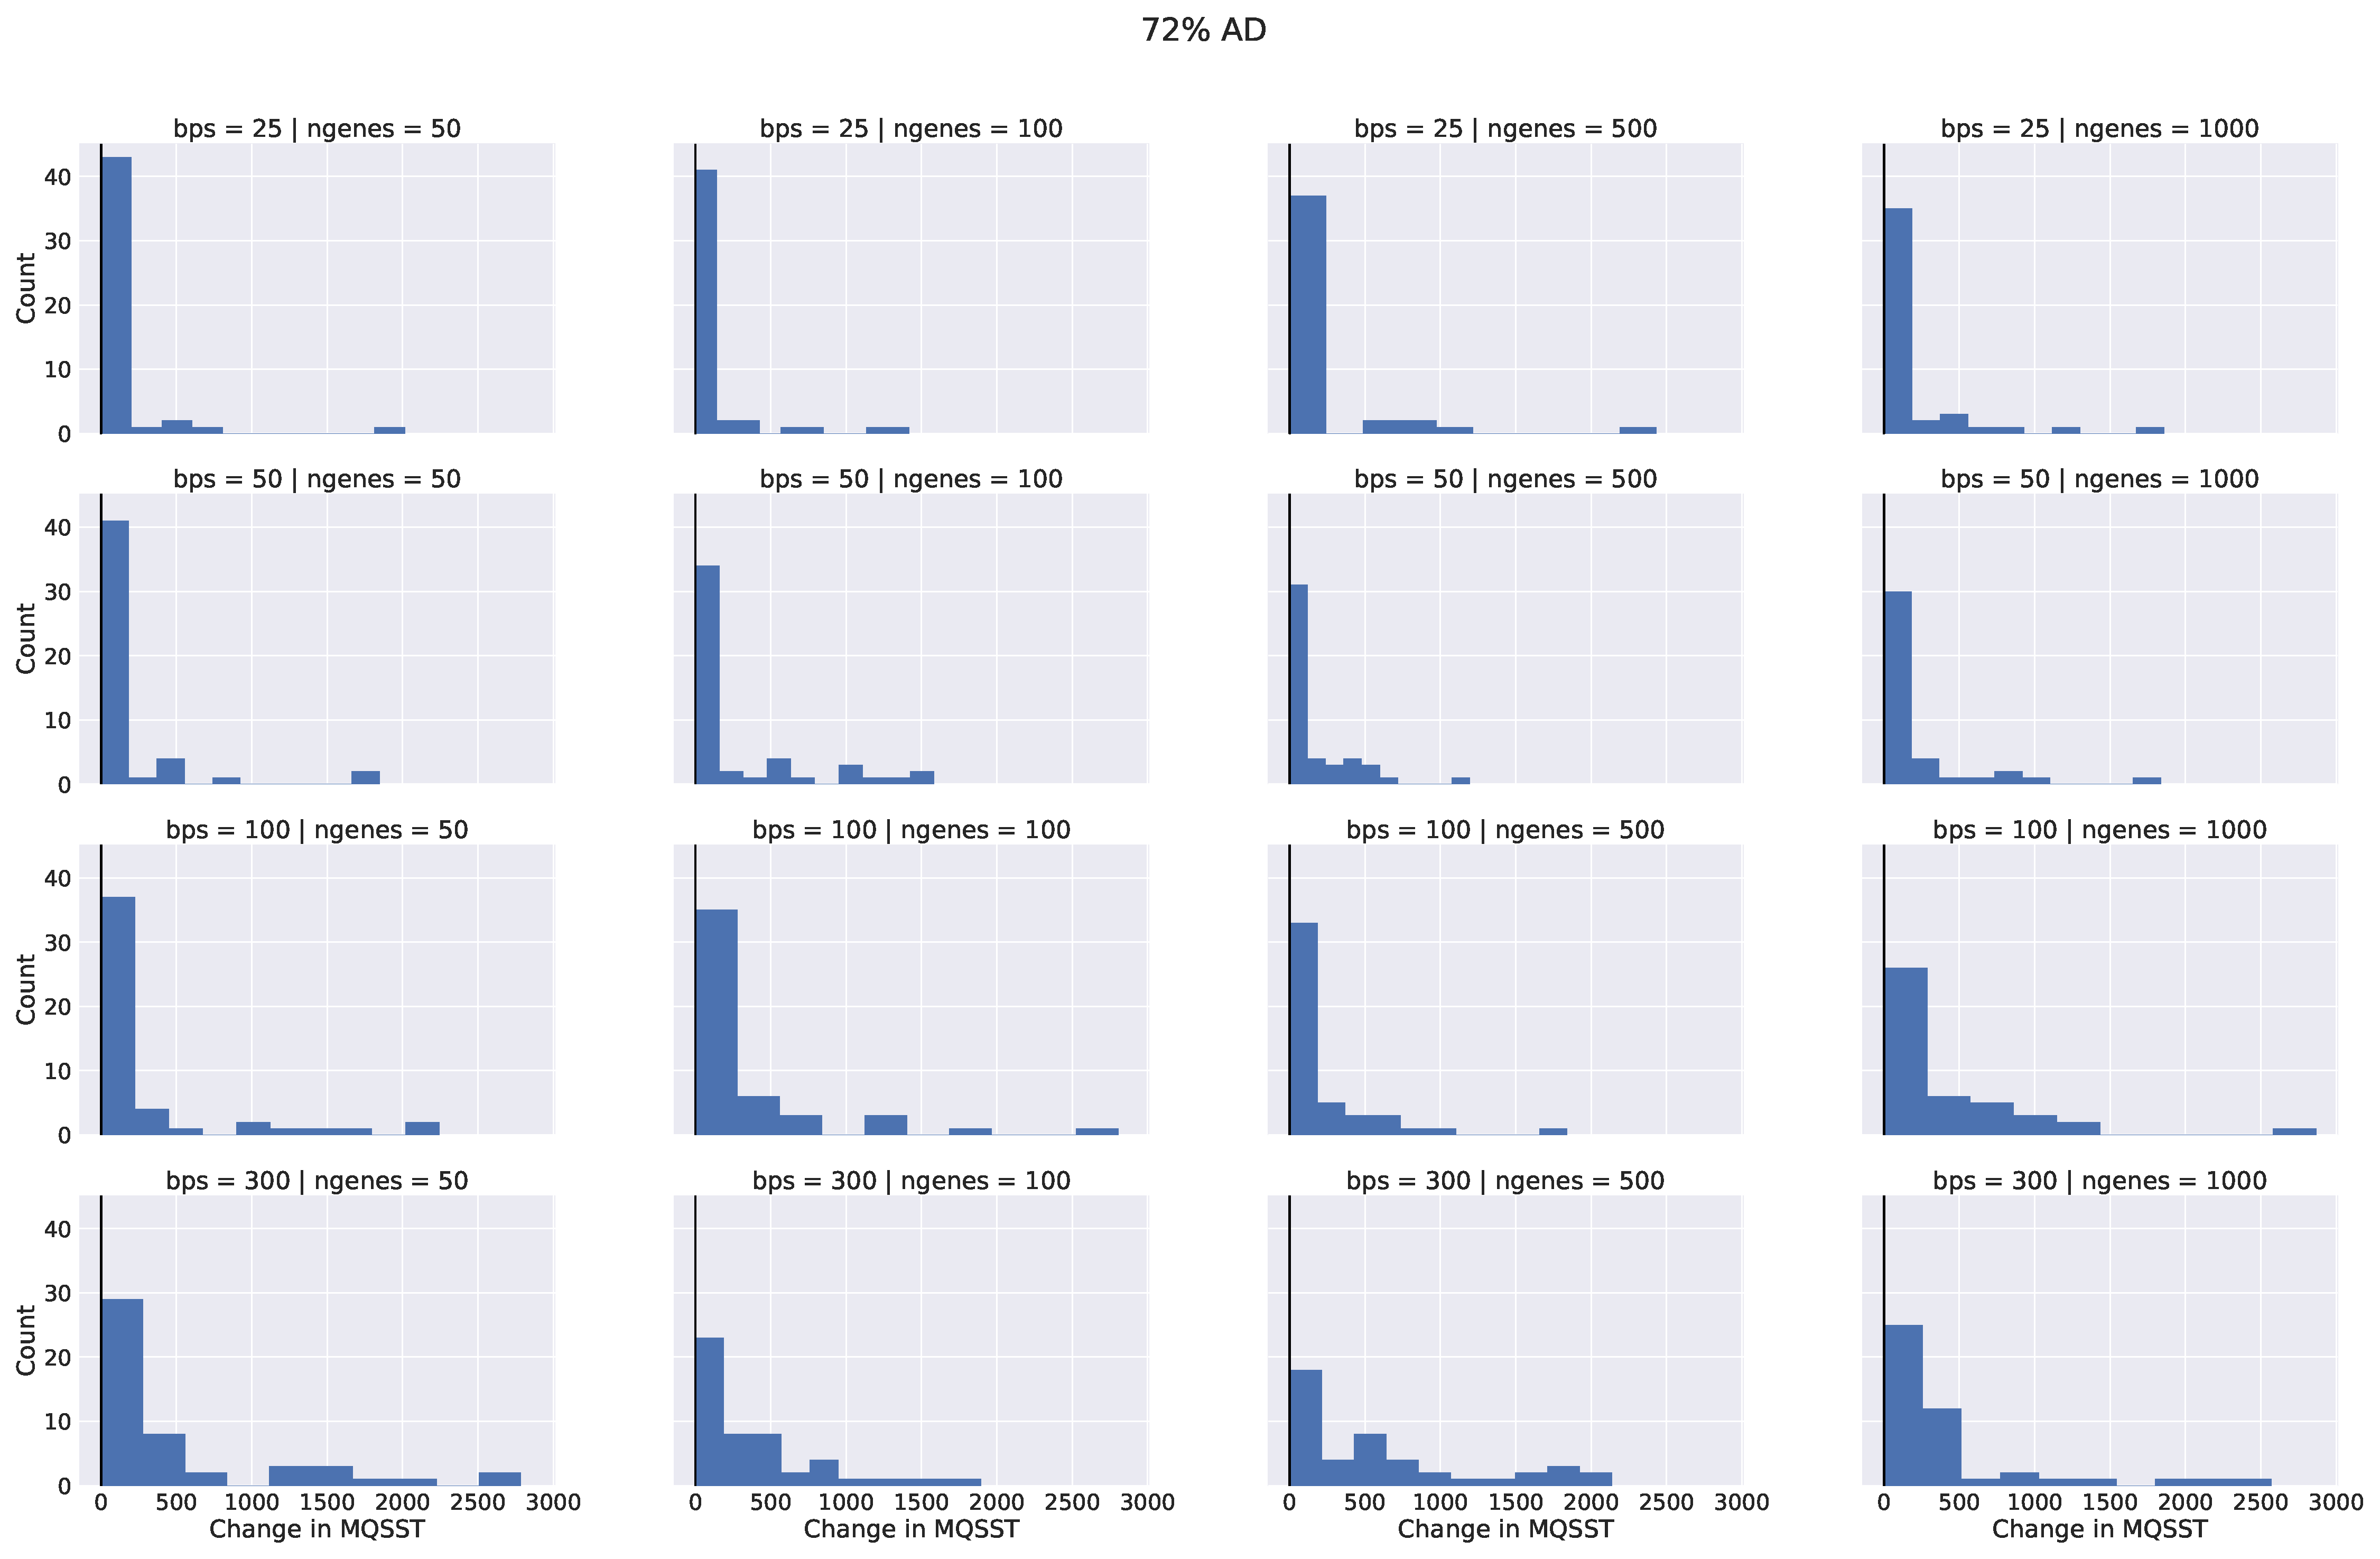
\includegraphics[width=\textwidth]{svdquest-figs/all-scorediffs-hist-cgenes-72.eps}
\caption[Histogram of differences in MQSST scores between SVDquartets+PAUP* and SVDquest*  for the very high ILS 50-taxon datasets]{Histogram of the difference in MQSST scores between
  SVDquartets+PAUP* and SVDquest*  on very high ILS (AD = 72\%) 50-taxon c-gene data
  with 40-50 replicates per model condition (i.e. a specific combination of ILS level, number of genes, and sequence length). Positive x-values
  indicate that SVDquest* finds a larger MQSST score than
  SVDquartets+PAUP*.
}
\label{fig:s3}
\end{figure}

\clearpage
\begin{figure}
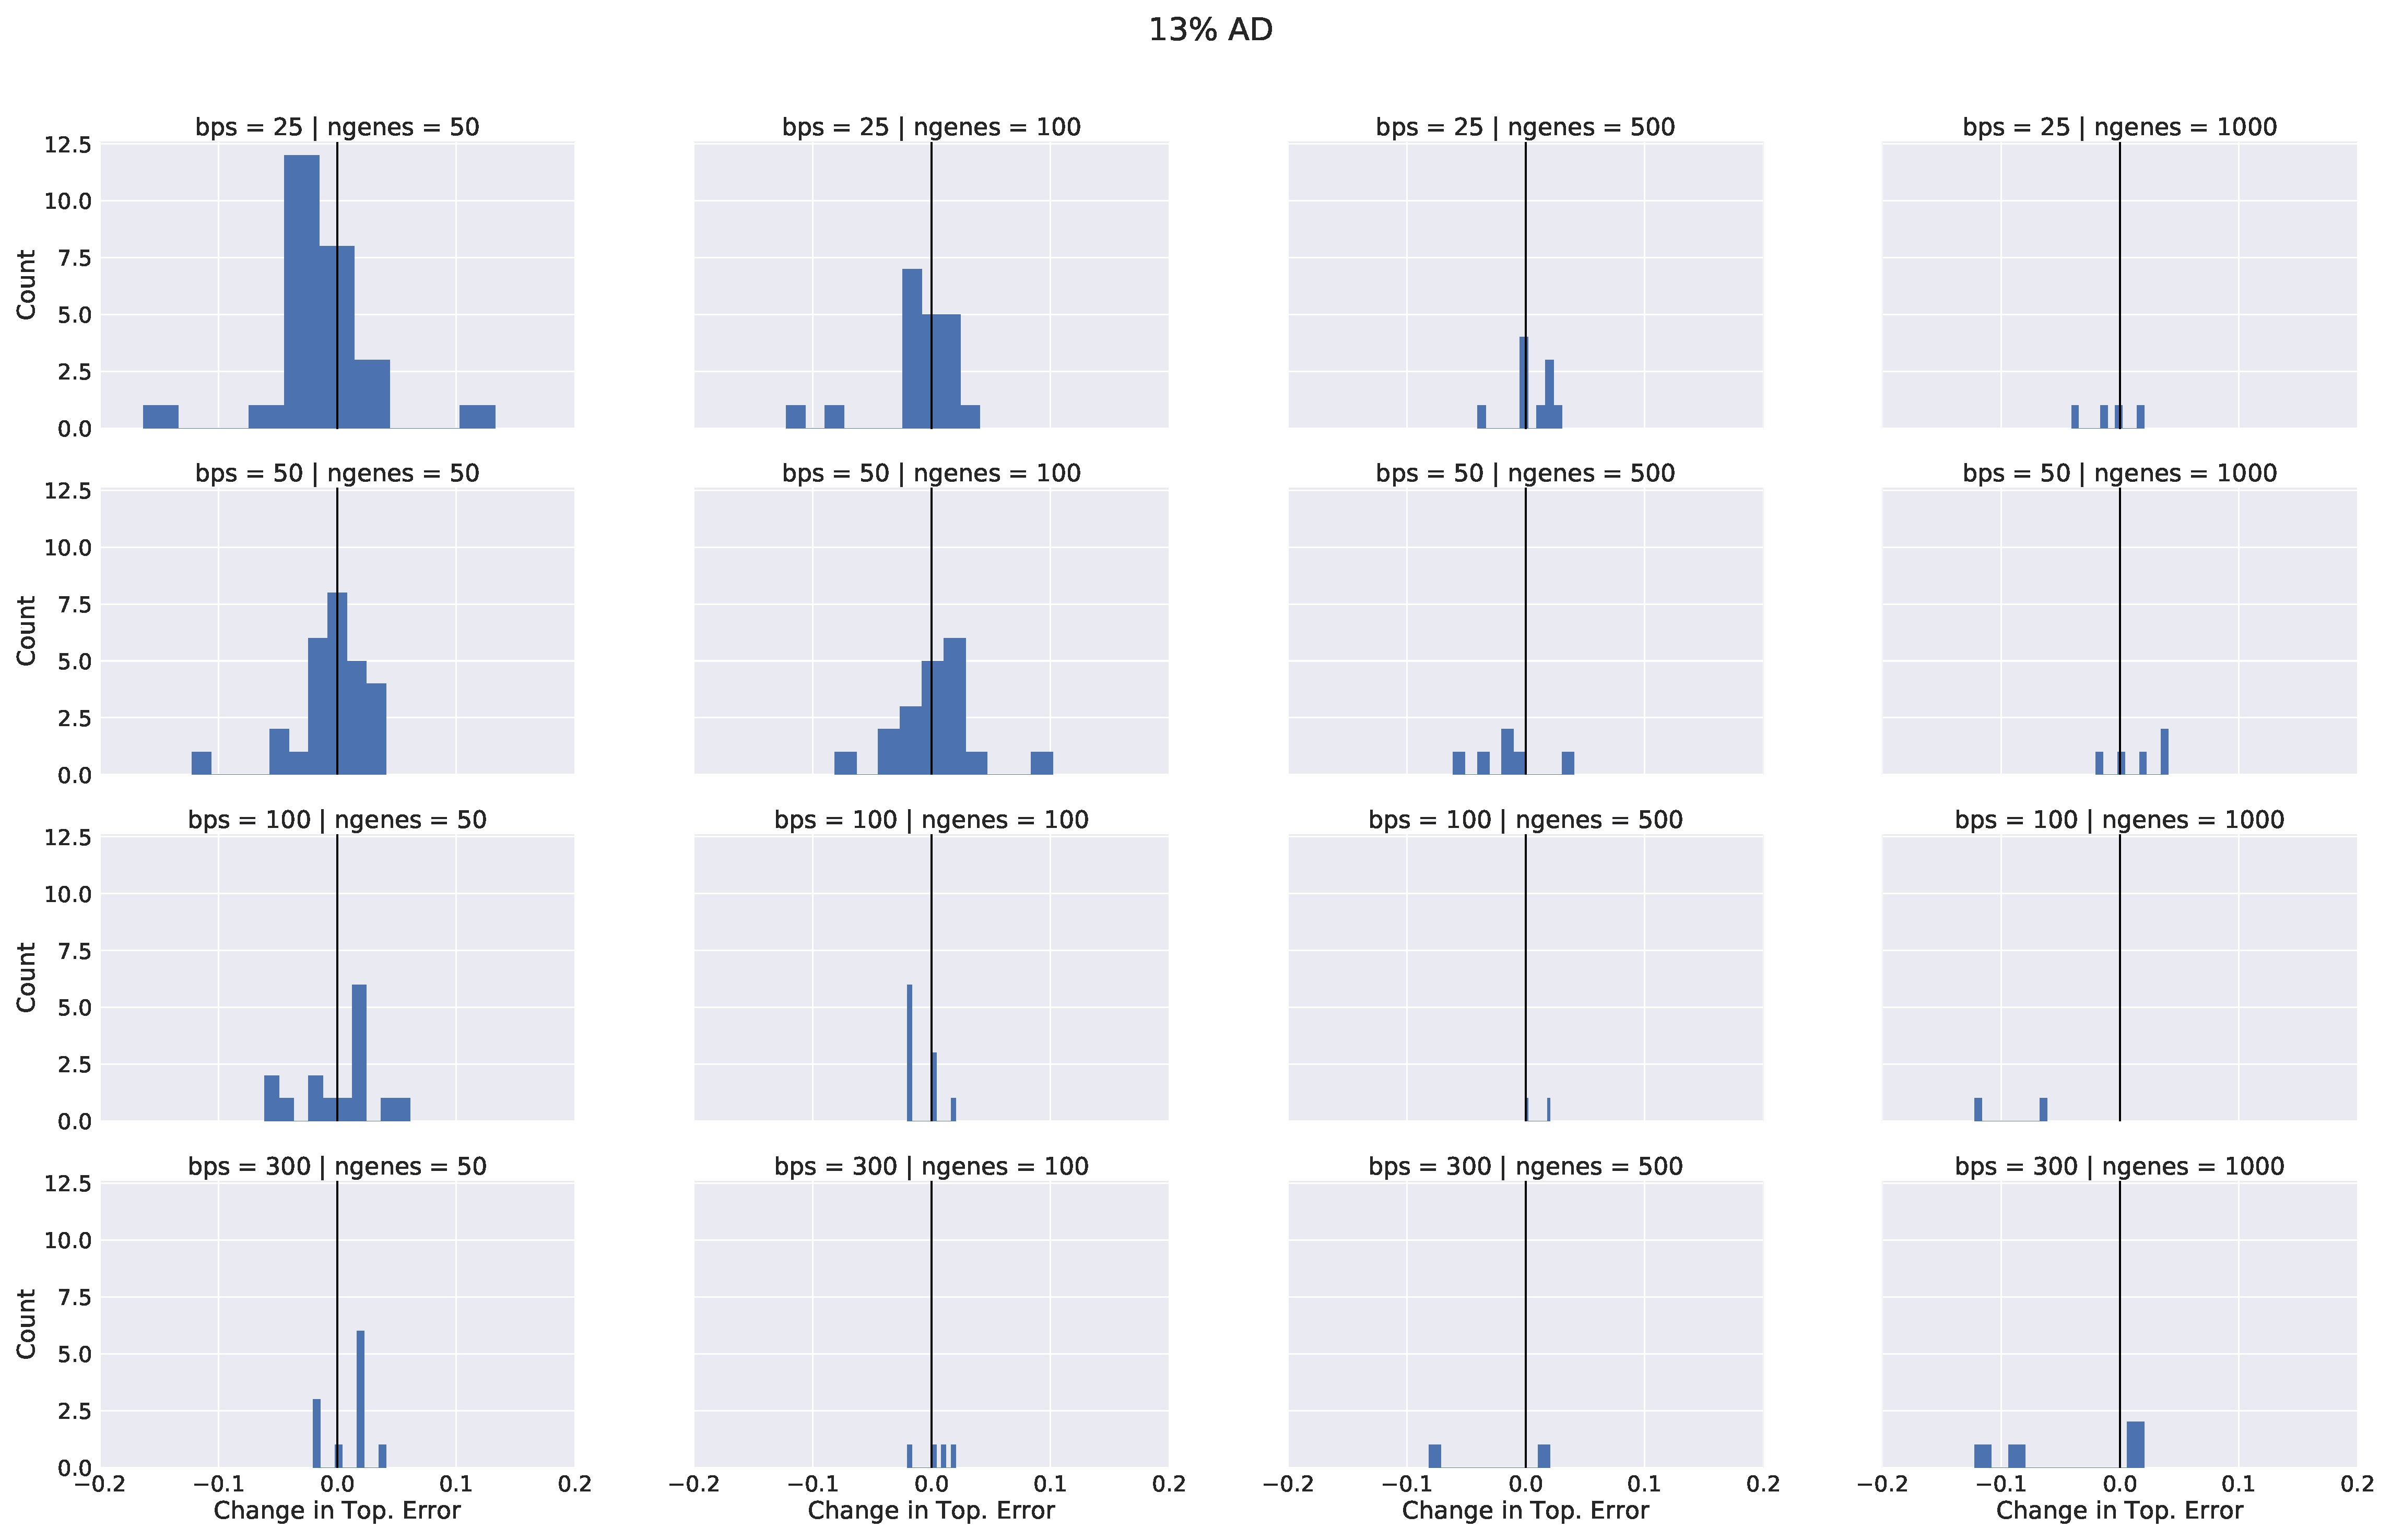
\includegraphics[width=\textwidth]{svdquest-figs/differentscore-rfdists-hist-cgenes-13.eps}
\caption[Histogram of differences in topological error between SVDquartets+PAUP* and SVDquest*-strict for the low ILS 50-taxon datasets]
{Histogram of the difference in topological error rates (maximum is 1.0) between
  SVDquartets+PAUP* and SVDquest*-strict (in the cases where SVDquartets+PAUP* and SVDquest* find trees
  with different MQSST scores)  for the low ILS (AD=13\%) 50-taxon data
  with 40-50 replicates per model condition (i.e. a specific combination of ILS level, number of genes, and sequence length). 
  Negative x-values indicate that SVDquest*-strict finds a topologically more accurate tree than
  SVDquartets+PAUP*.
When SVDquest* found a better MQSST score than SVDquartets+PAUP*, SVDquest*-strict was more
accurate  40\% of the time, equally accurate 24\% of the time, and
less accurate 35\% of the time.
%When SVDquest* and SVDquartets+PAUP* found  the same MQSST score, SVDquest*-strict was more accurate 5\% of the time, equally accurate 92\% of the time, and less accurate 3\% of the time.
}
\label{fig:s4}
\end{figure}




\clearpage

\begin{figure}
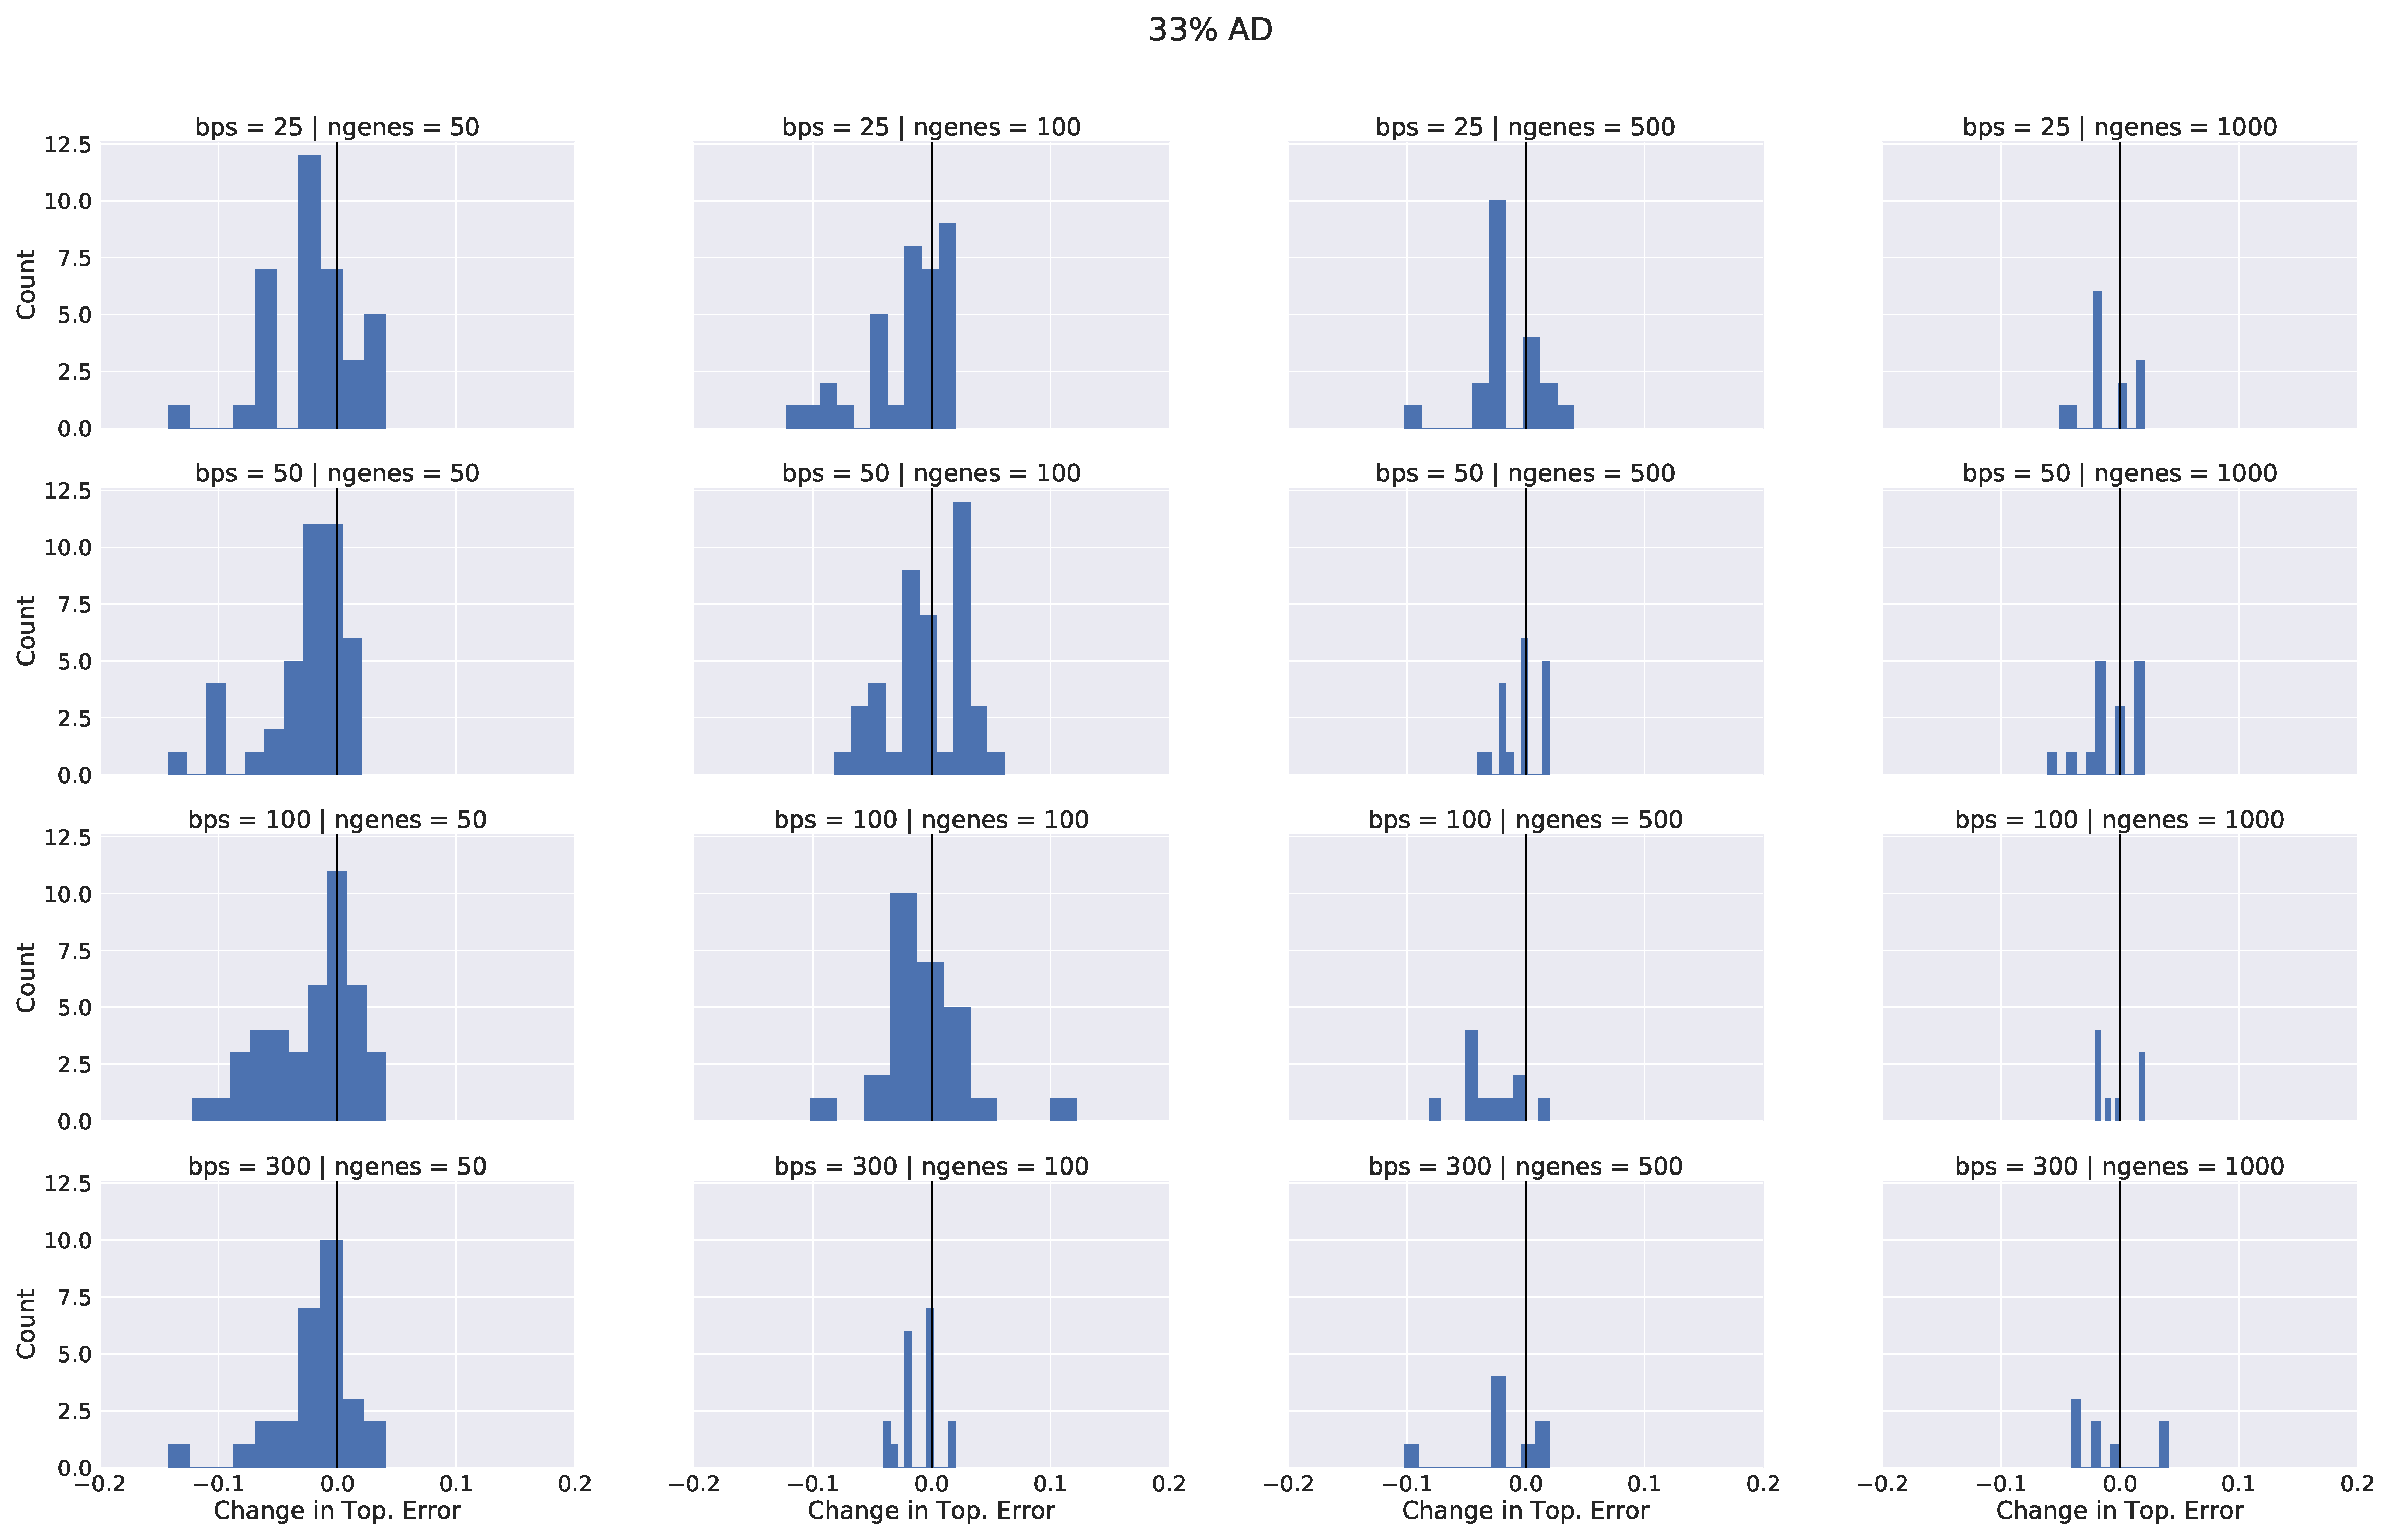
\includegraphics[width=\textwidth]{svdquest-figs/differentscore-rfdists-hist-cgenes-33.eps}
\caption[Histogram of differences in topological error between SVDquartets+PAUP* and SVDquest*-strict for the high ILS 50-taxon datasets]{Histogram of the difference in topological error rates (maximum is 1.0) between
  SVDquartets+PAUP* and SVDquest*-strict (in the cases where SVDquartets+PAUP* and SVDquest* find trees
  with different MQSST scores)  on high ILS (AD = 33\%) 50-taxon data with
  40-50 replicates per model condition (i.e. a specific combination of ILS level, number of genes, and sequence length). 
  Negative x-values indicate
  that SVDquest*-strict finds a topologically more accurate tree than SVDquartets+PAUP*.
  When SVDquest* found a better scoring tree than SVDquartets+PAUP*, SVDquest*-strict was more
accurate   52\% of the time, equally accurate 24\% of the time, and
less accurate 23\% of the time.
%When SVDquest* and SVDquartets+PAUP* found trees with the same score, SVDquest*-strict was more accurate 3\% of the time, equally accurate 93\% of the time, and less accurate 4\% of the time.
}
\label{fig:s5}
\end{figure}




\clearpage

\begin{figure}
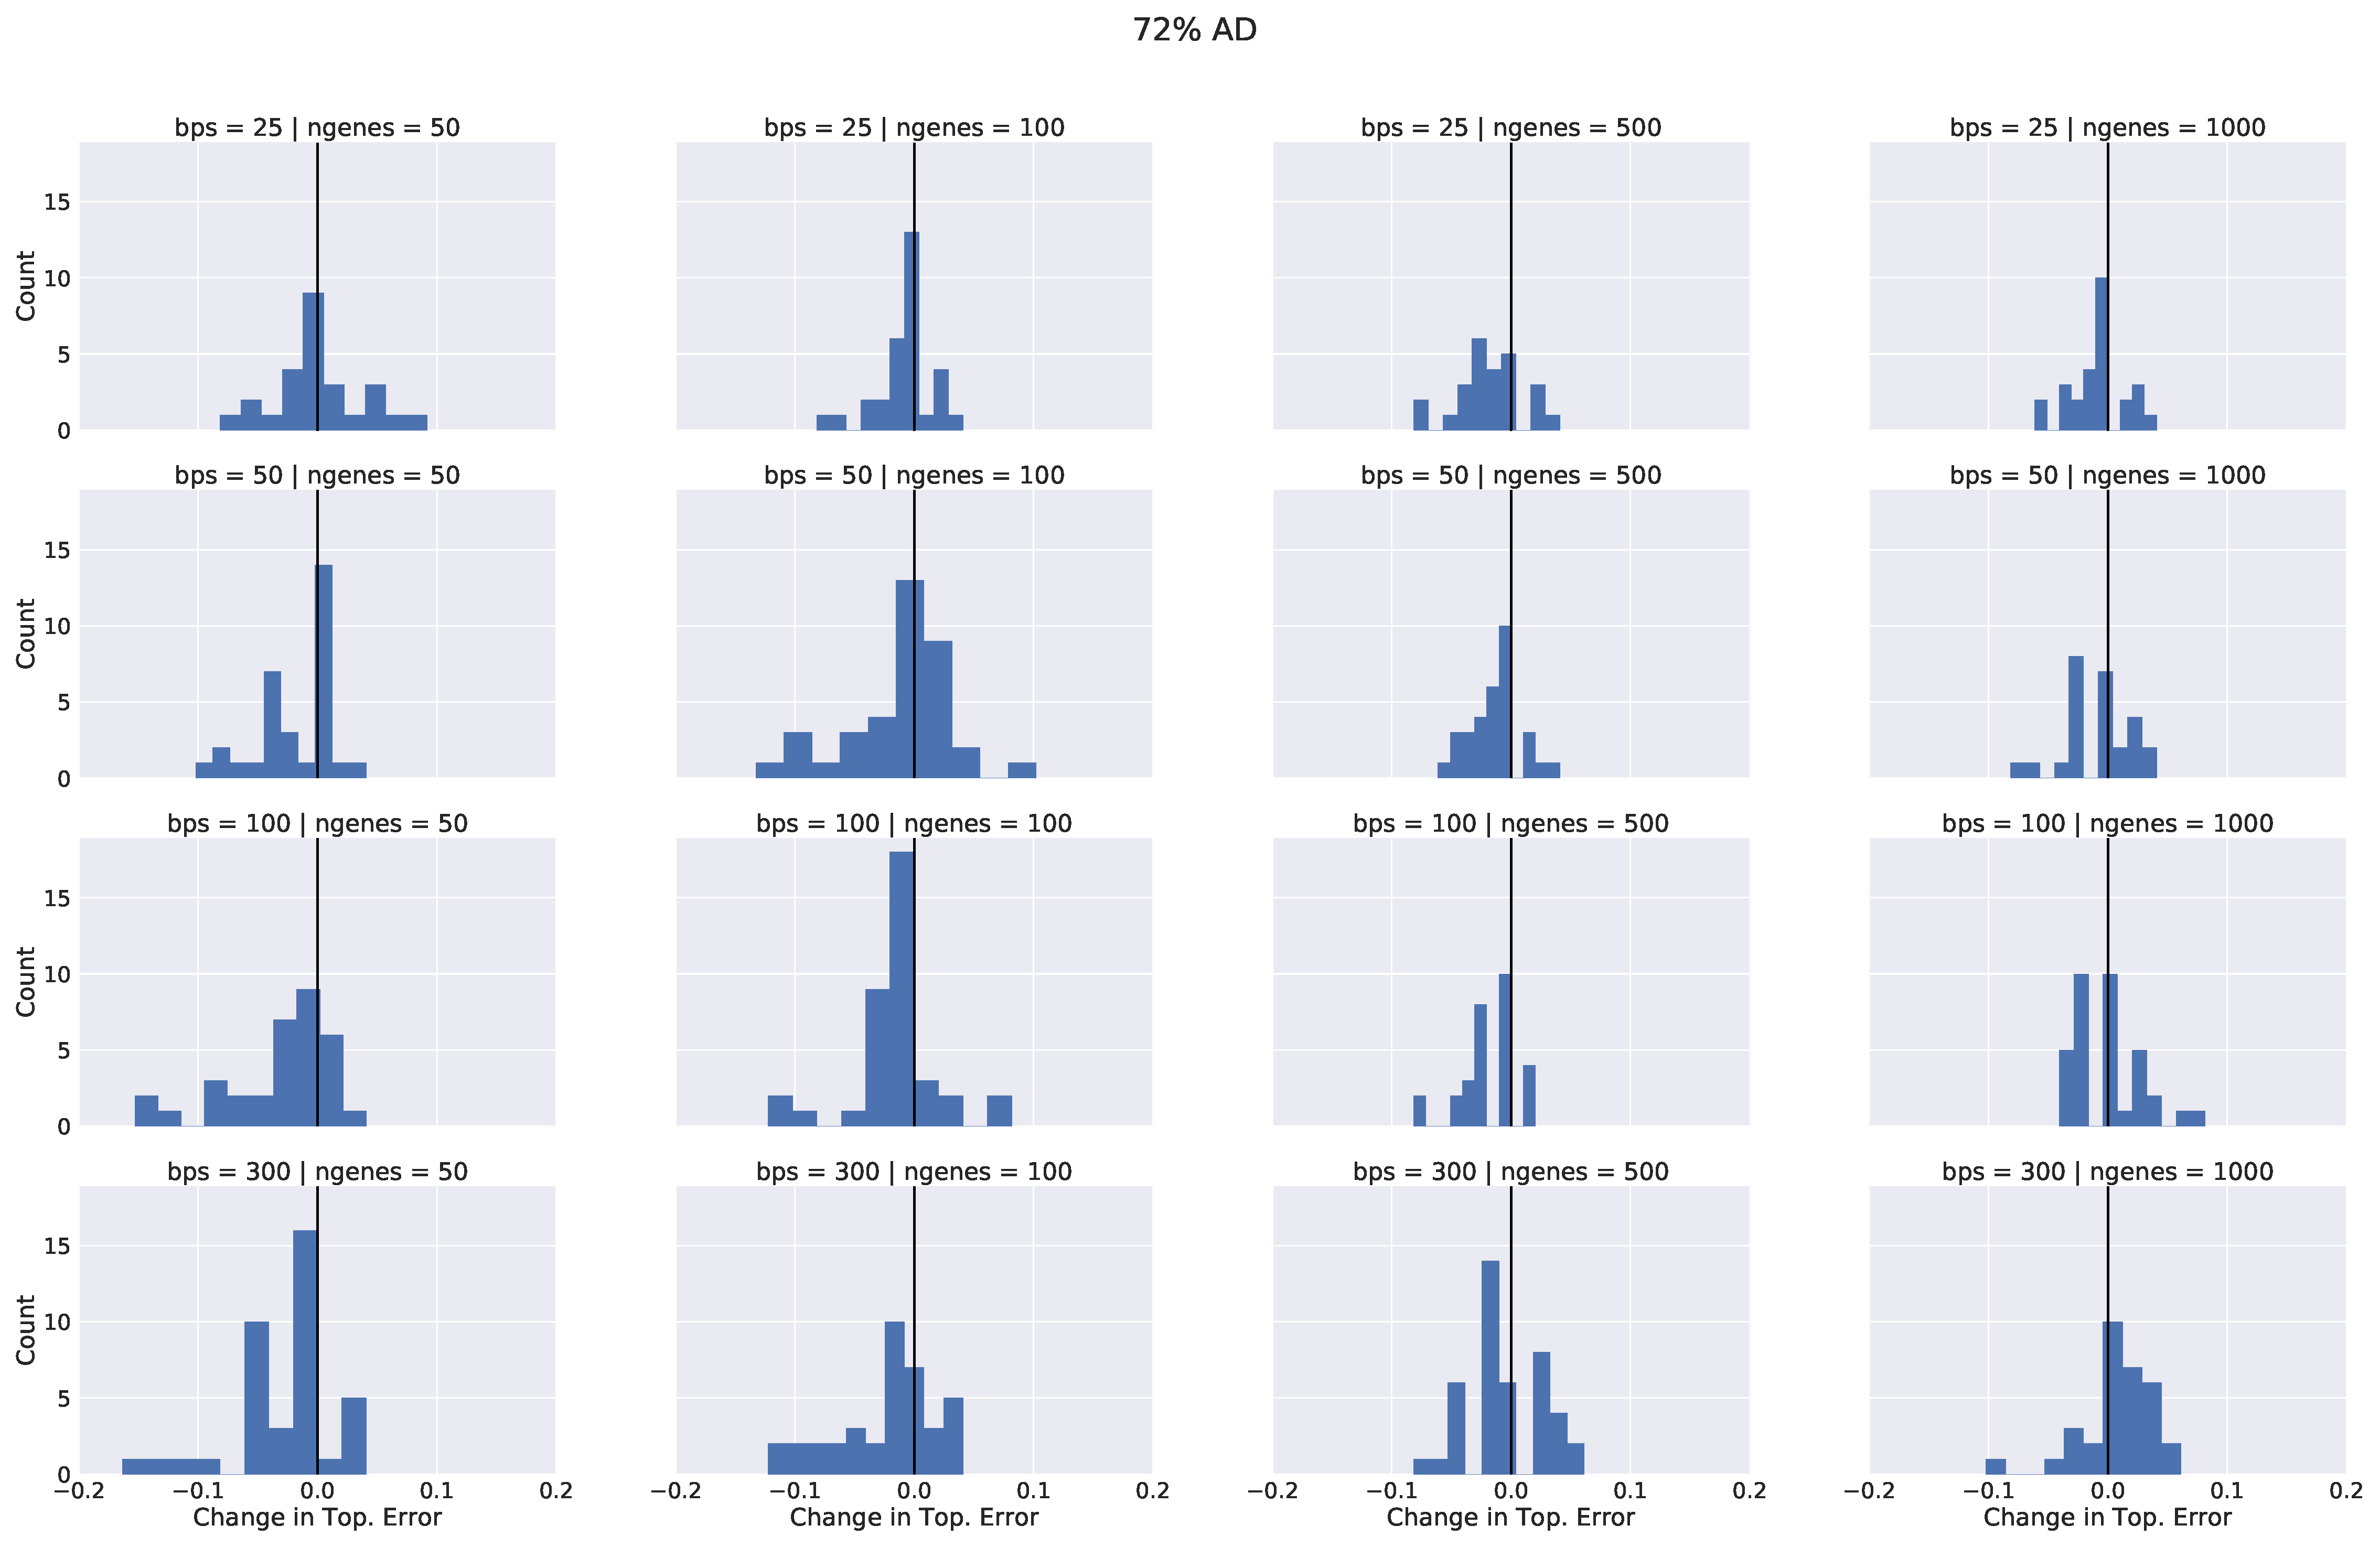
\includegraphics[width=\textwidth]{svdquest-figs/differentscore-rfdists-hist-cgenes-72.eps}
\caption[Histogram of differences in topological error between SVDquartets+PAUP* and SVDquest*-strict for the very high ILS 50-taxon datasets]{Histogram of the difference in topological error rates (maximum is 1.0)  between
  SVDquartets+PAUP* and SVDquest*-strict (in the cases where SVDquartets+PAUP* and SVDquest* find trees
  with different MQSST scores)   on very high ILS (AD = 72\%) 50-taxon data
  with 40-50 replicates per model condition (i.e. a specific combination of ILS level, number of genes, and sequence length). 
  Negative x-values 
  indicate that SVDquest*-strict finds a topologically more accurate tree than
  SVDquartets+PAUP*.
When SVDquest* found a better MQSST score  than SVDquartets+PAUP*, SVDquest*-strict was a more
accurate tree 51\% of the time, equally accurate 27\% of the time, and
less accurate 21\% of the time.
%When SVDquest* and SVDquartets+PAUP* found  the same MQSST score, SVDquest*-strict was more accurate 10\% of the time, equally accurate 75\% of the time, and less accurate 15\% of the time.
}
\label{fig:s6}
\end{figure}

\clearpage





\clearpage

\begin{figure}
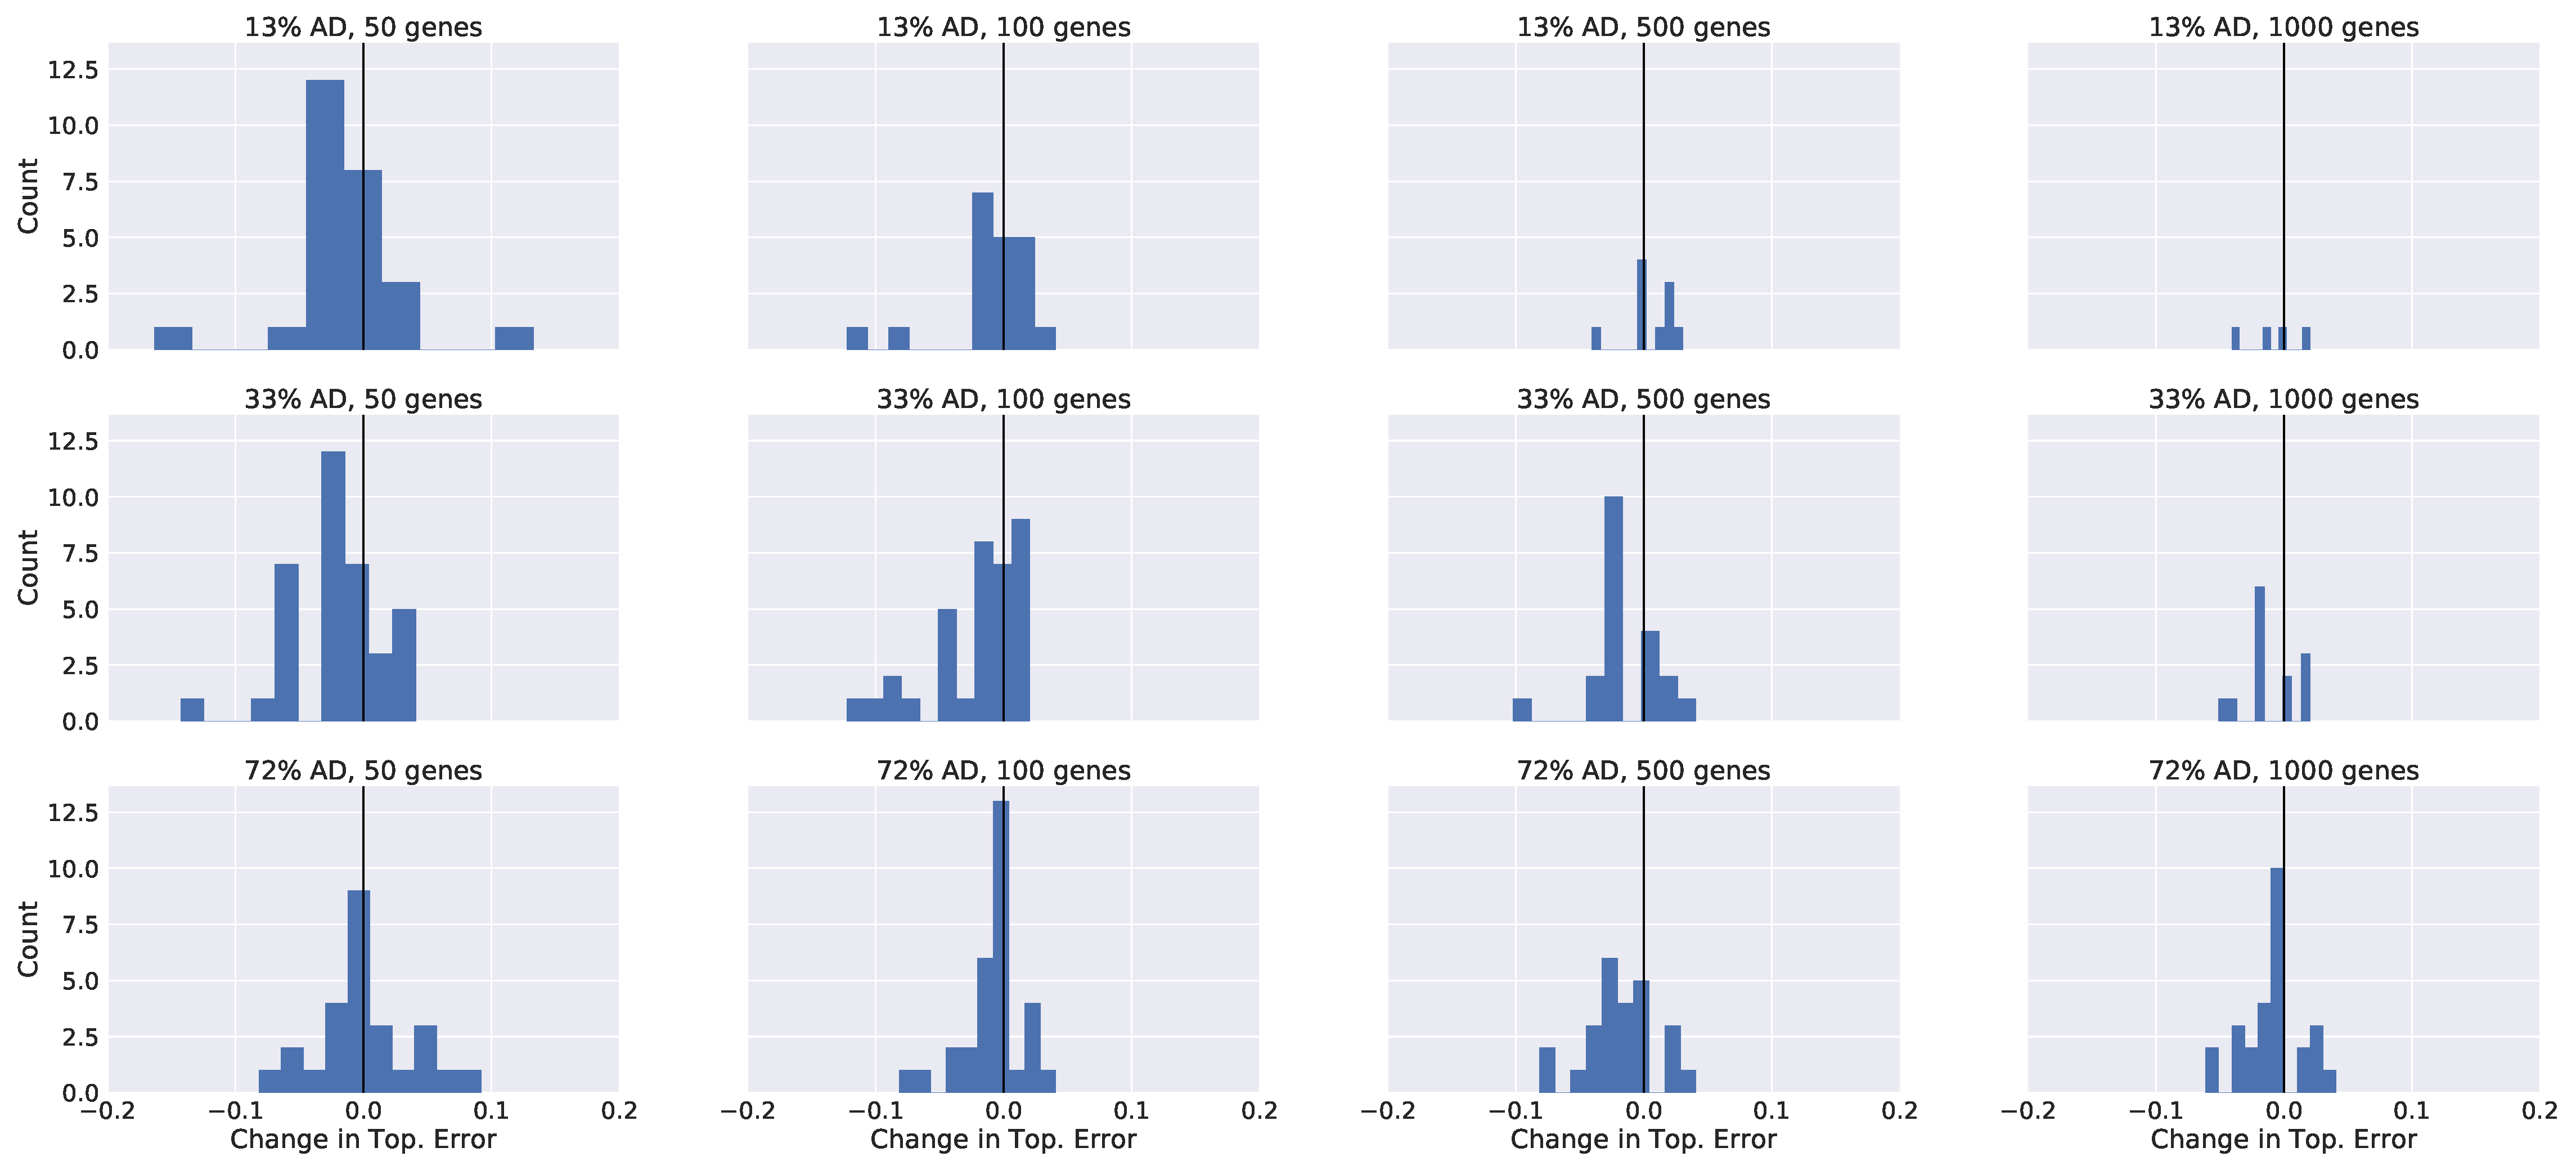
\includegraphics[width=\textwidth]{svdquest-figs/differentscore-rfdists-hist-cgenes-25bps.eps}
\caption[Histogram of differences in topological error rates between SVDquartets+PAUP* and SVDquest*-strict for the 25-site 50-taxon datasets]{Histogram of the difference in topological error rates (maximum is 1.0)  between
  SVDquartets+PAUP* and SVDquest*-strict (in the cases where SVDquartets+PAUP* and SVDquest* find trees with different MQSST scores)  25-site c-gene 50-taxon data
  with 40-50 replicates per model condition (i.e. a specific combination of ILS level, number of genes, and sequence length). 
  Negative x-values 
  indicate that SVDquest*-strict finds a topologically more accurate tree than
  SVDquartets+PAUP*.}
  \label{fig:s7}
\end{figure}

%\clearpage
%\begin{figure}
 % 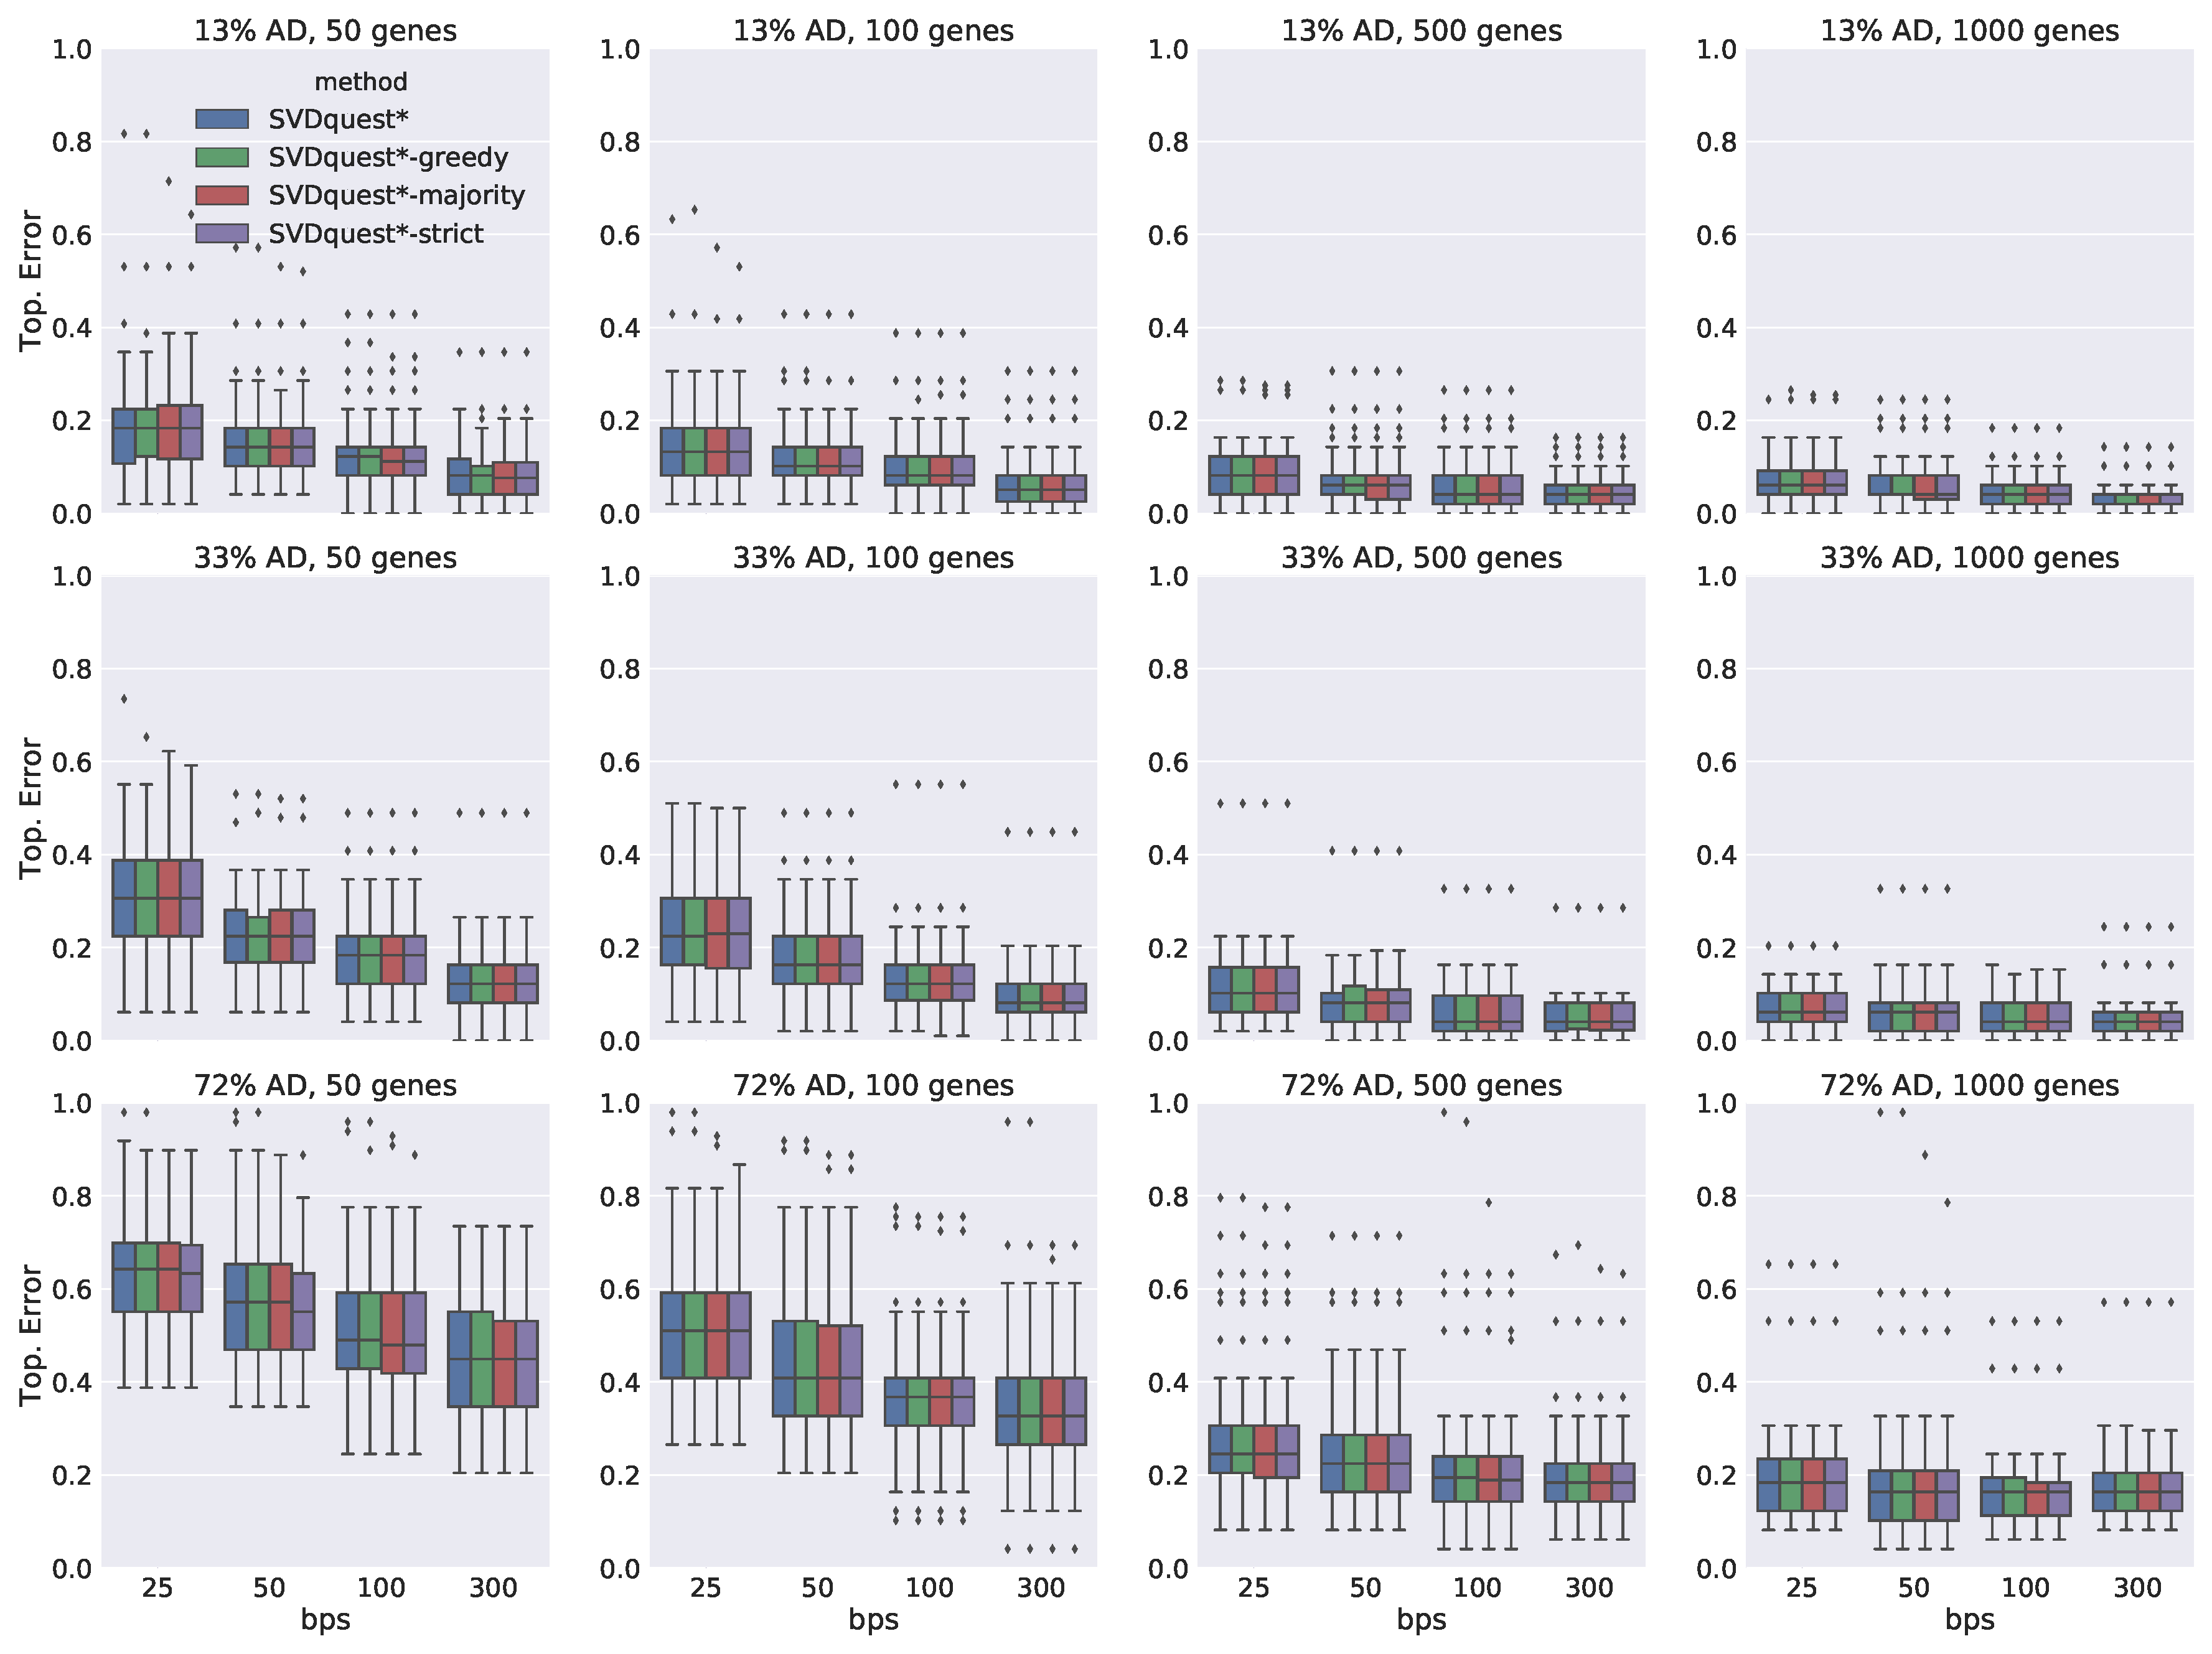
\includegraphics[width=\textwidth]{cgene-siesta.eps}
 % \caption[Species tree error rates for different consensus trees of the SVDquest* trees on 50-taxon datasets]{Species tree topological error rates (maximum is 1.0) for  different consensus trees (computed using SIESTA) of SVDquest*  trees on the 50-taxon c-gene data with 40-50 replicates per model condition.}
 % \label{fig:s8}
%\end{figure}

%\clearpage
%\begin{figure}
%  \centering
%  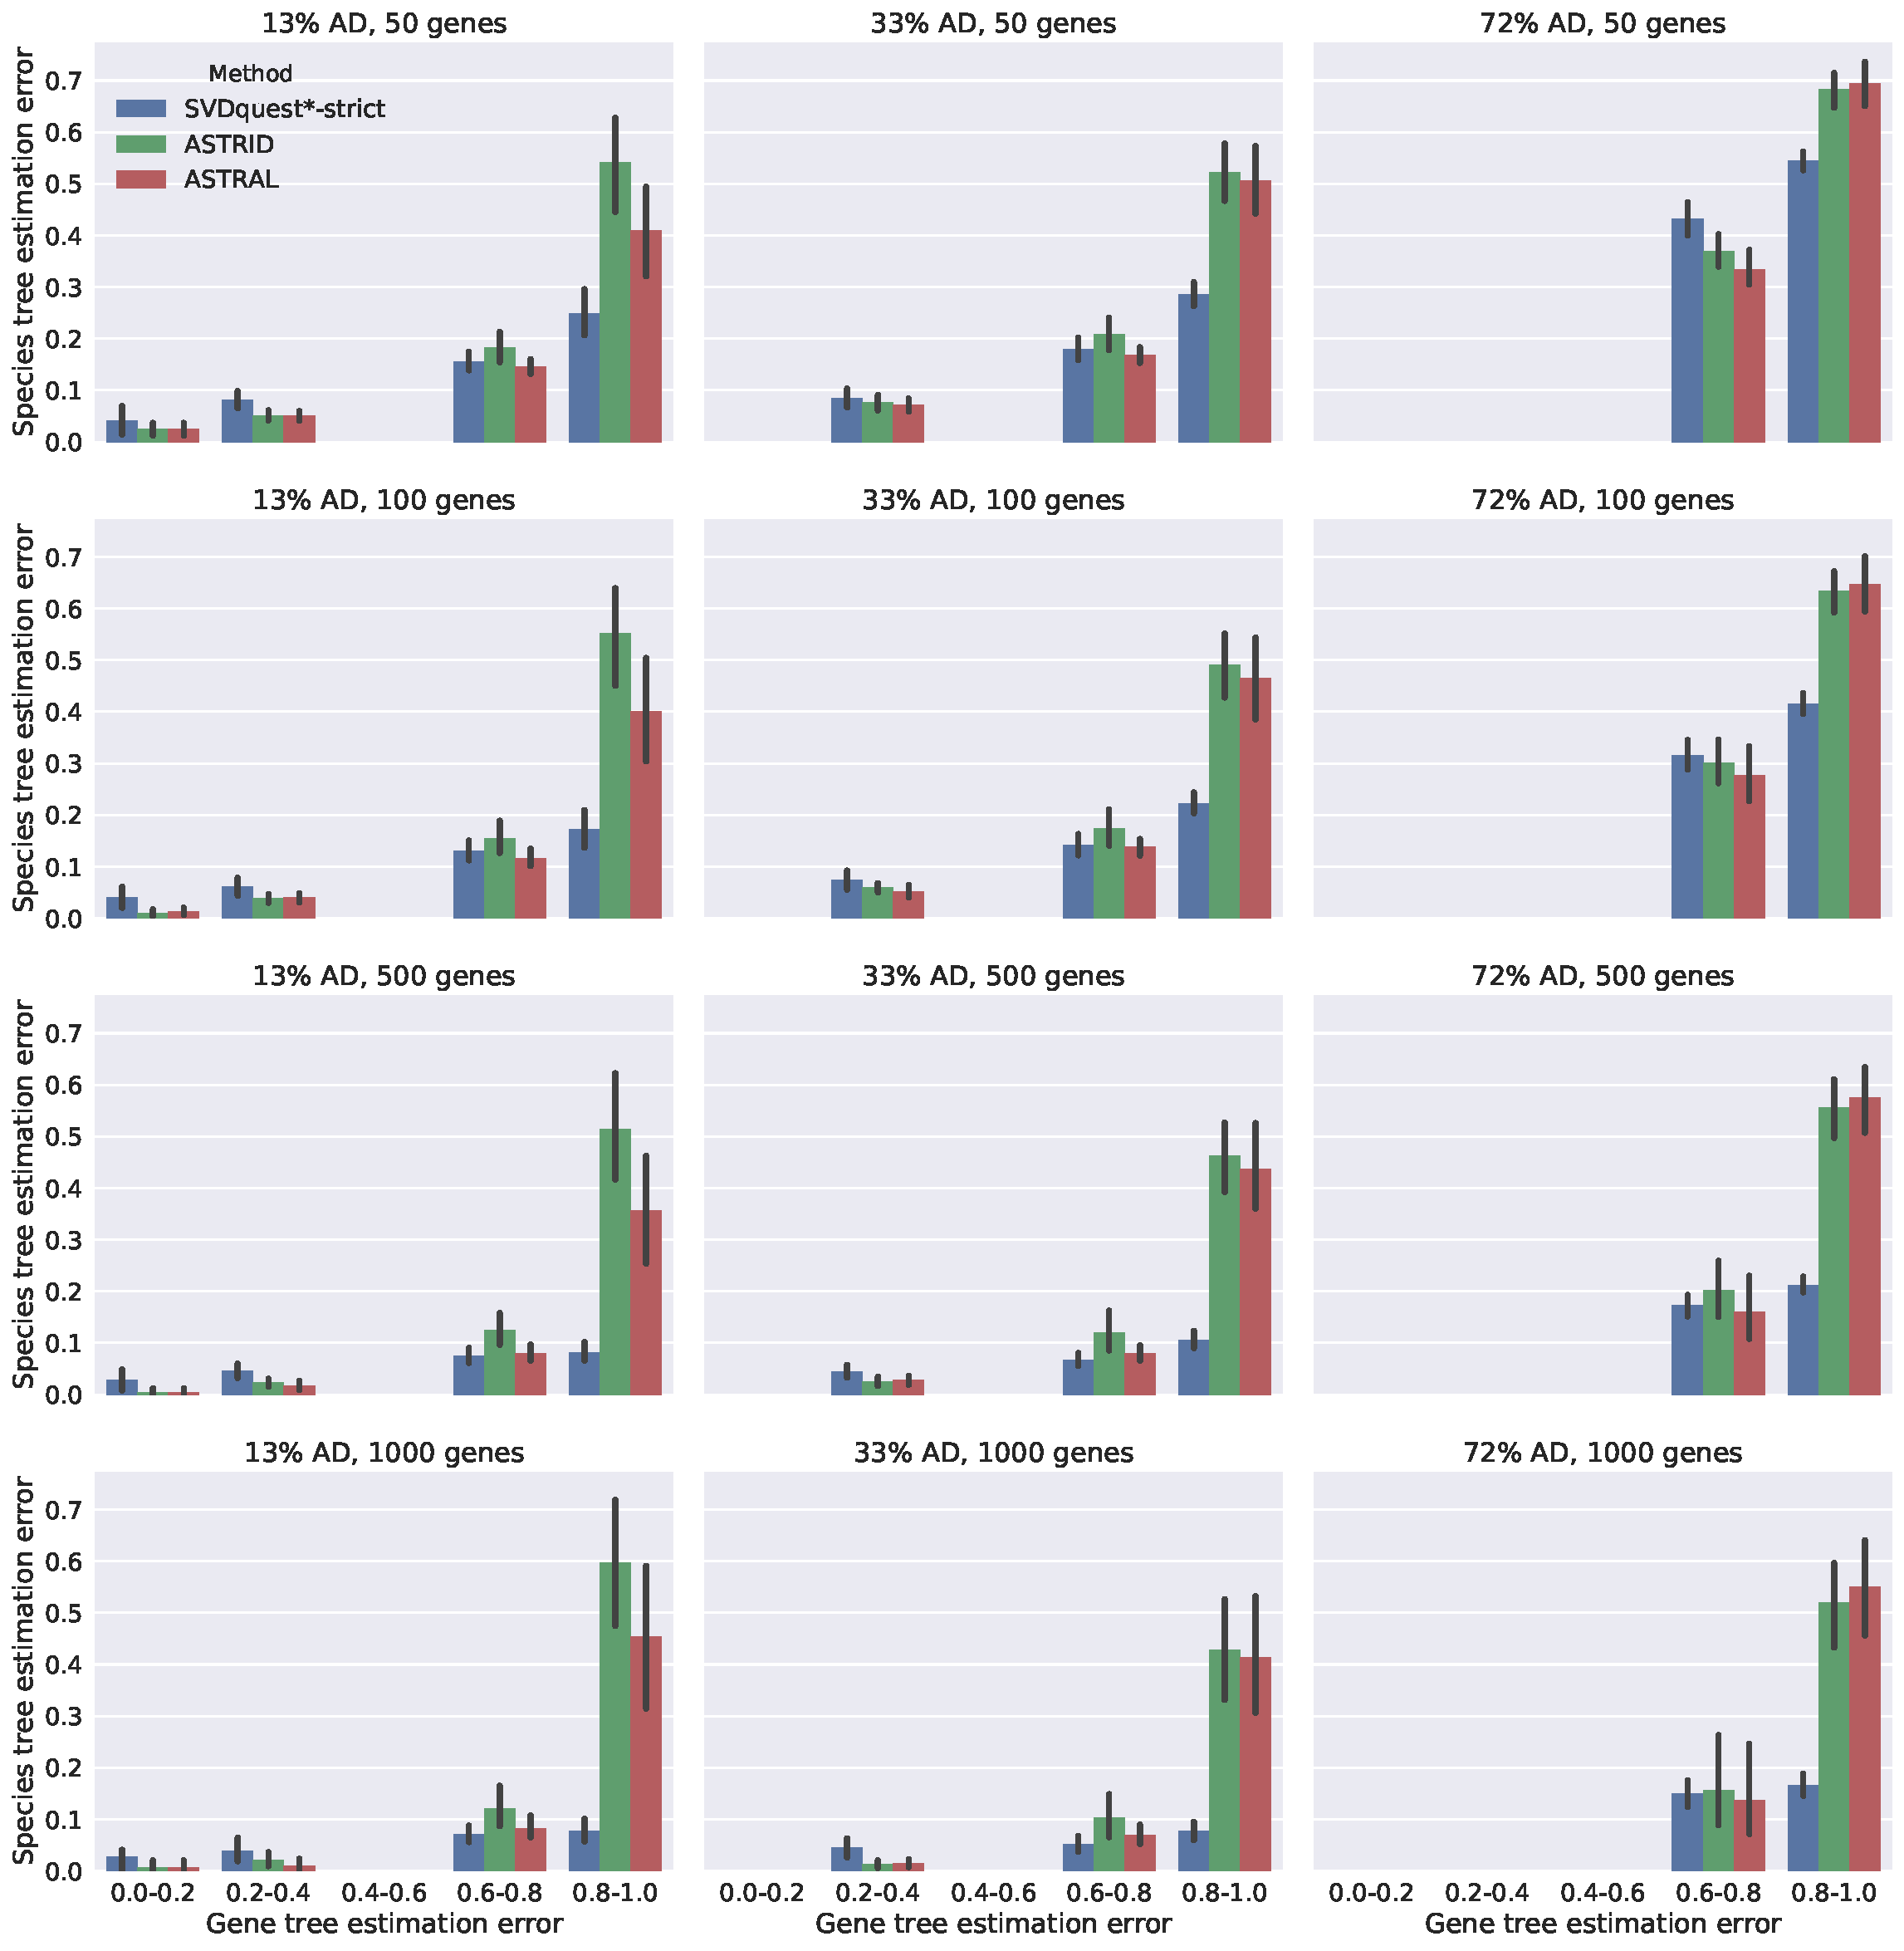
\includegraphics[width=\textwidth]{coalescent_rfdists_all.pdf}
%  \caption[Impact of gene tree estimation error on ASTRAL, ASTRID, and SVDquest*-strict on 50-taxon datasets]{Species tree topological error rates (maximum is 1.0) for ASTRAL, ASTRID, and SVDquest*-strict on 50-taxon simulated data, as a function of
%    gene tree estimation error (maximum is 1.0); each subfigure shows
%    results for 120-150 replicates. 
%    Error bars show standard error.    
%    }%\label{fig:exp2_50}
%    \label{fig:s9}
%    \end{figure}


\begin{figure}
  \centering
  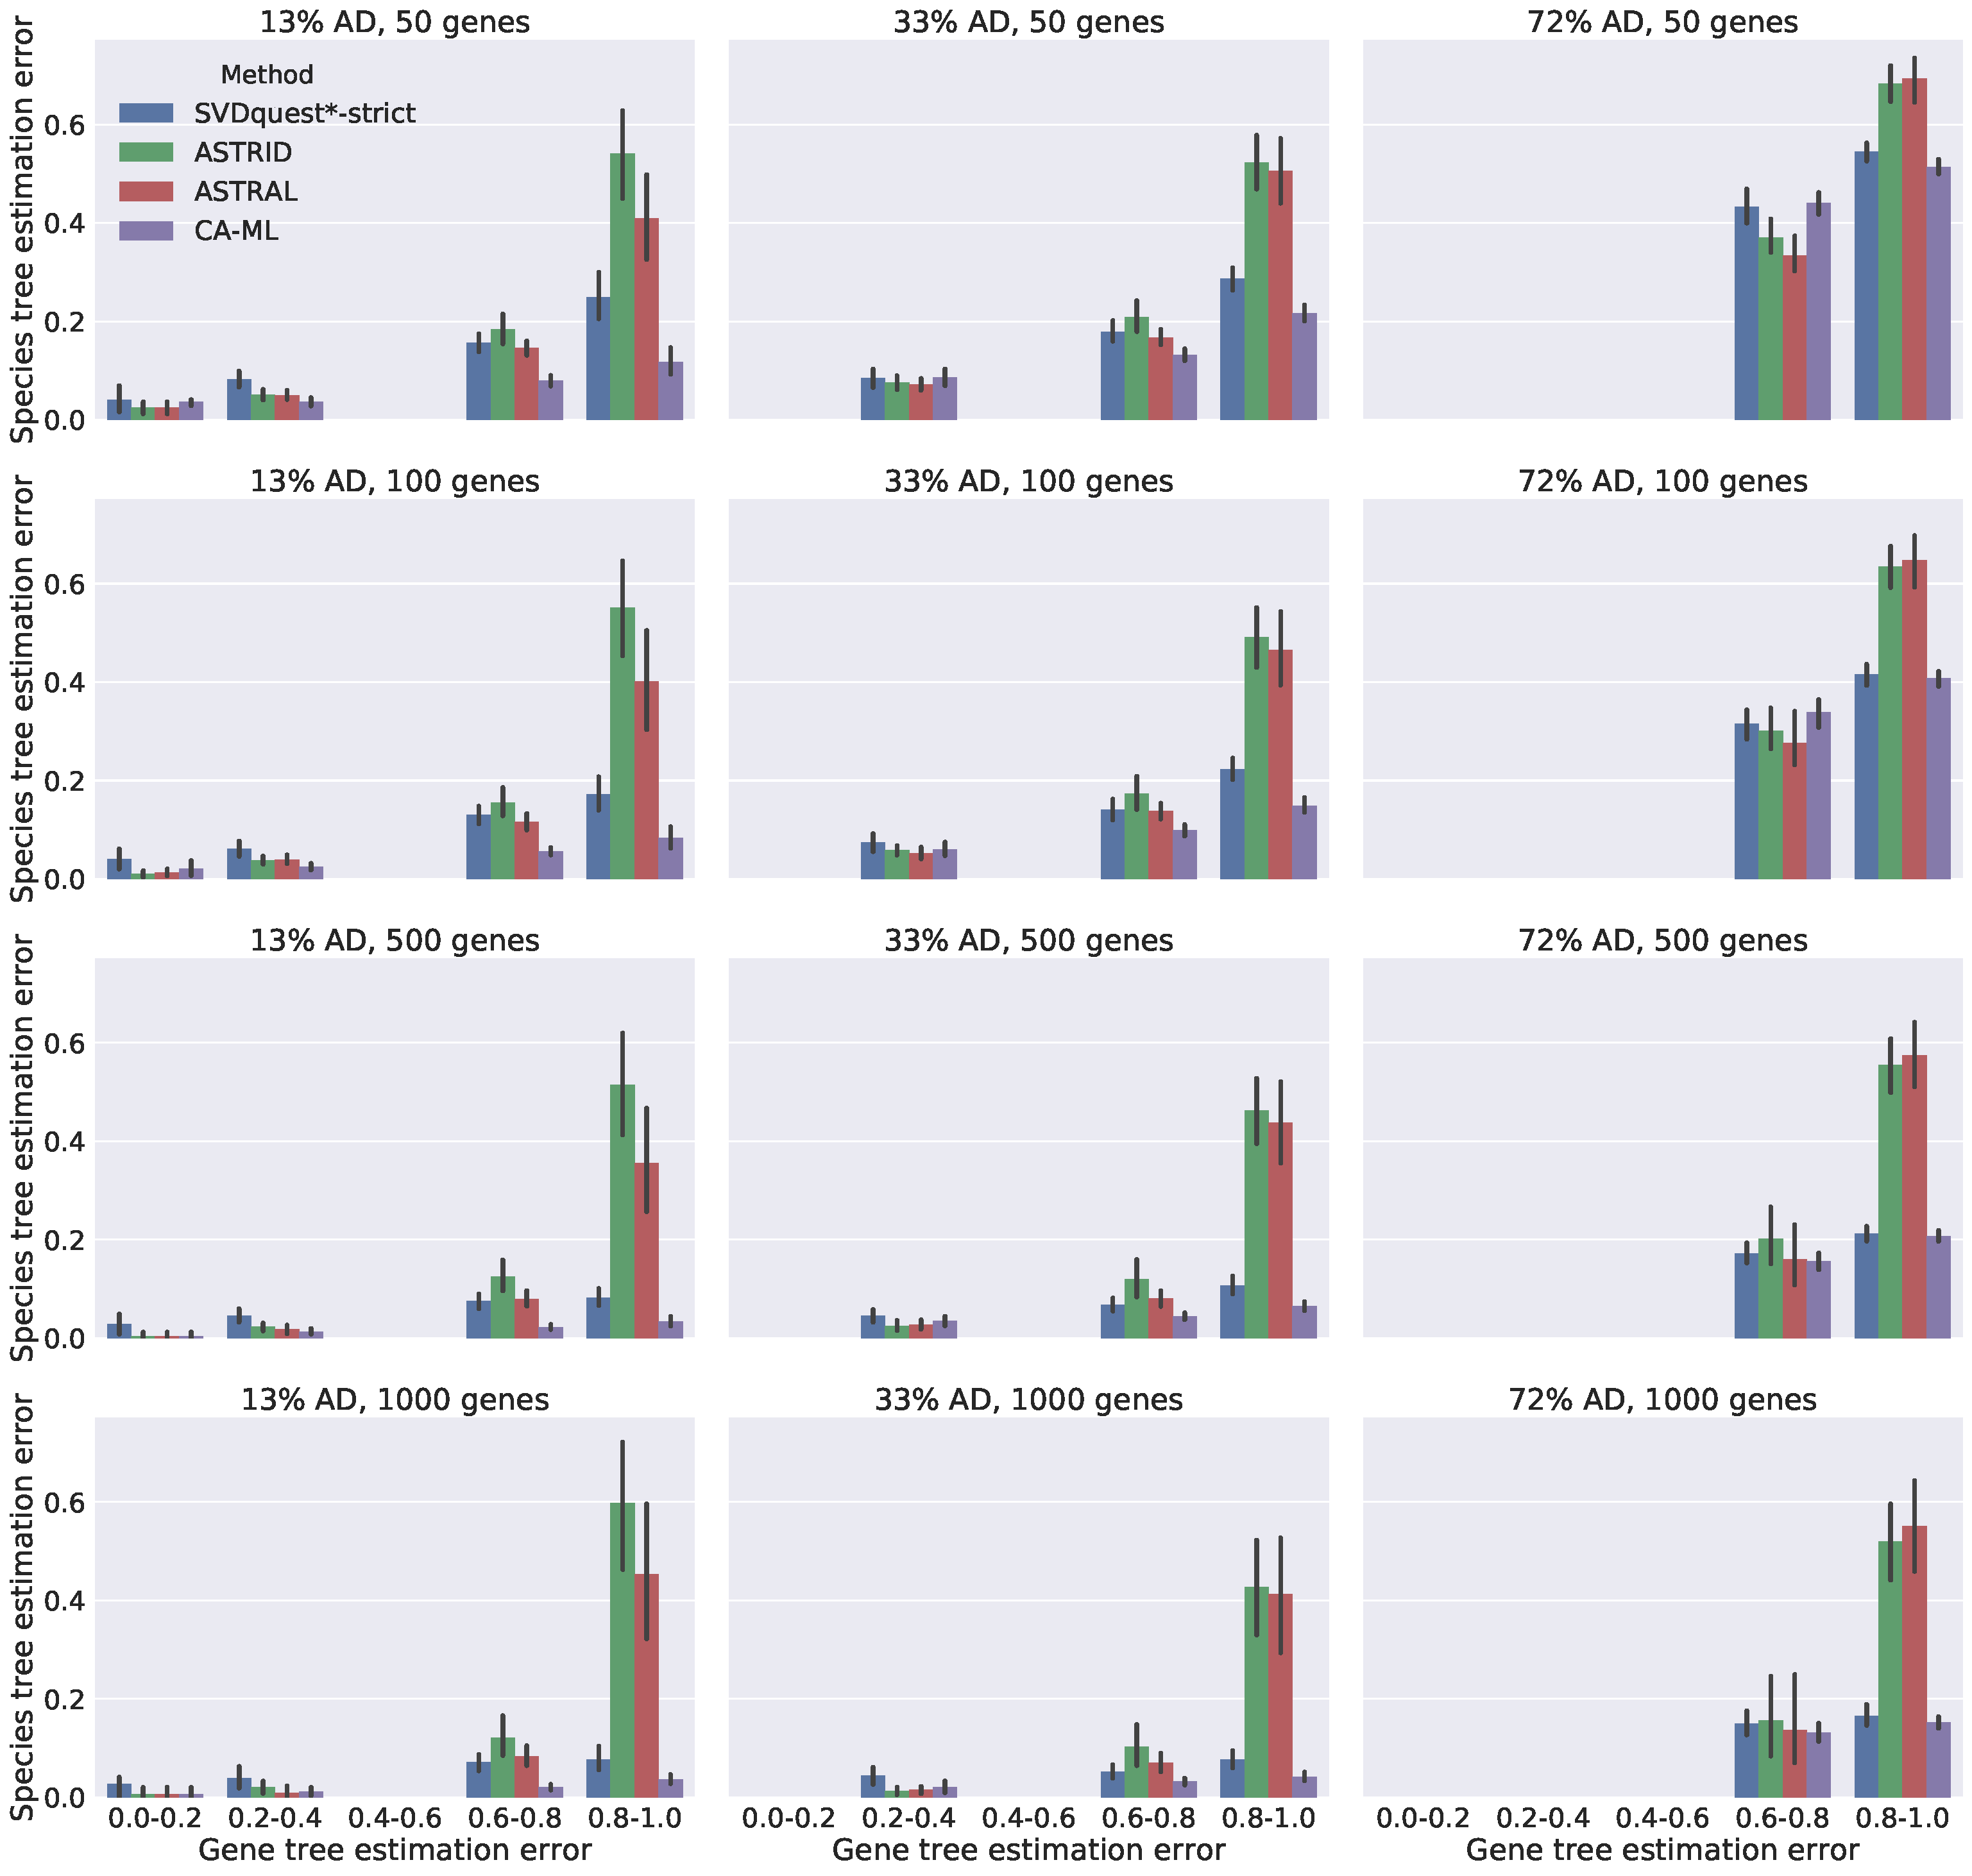
\includegraphics[width=\textwidth]{svdquest-figs/concat_rfdists_all.pdf}
\caption[Species tree error rates of SVDquest*-strict, ASTRID, ASTRAL, and CA-ML on 50-taxon supergene datasets]{Species tree topological error rates (maximum is 1.0) for 50-taxon simulated data, as a function of the normalized percent
    gene tree estimation error (maximum is 1.0), averaged over 120-150 replicates.
    Error bars show standard
    error.}
%\label{fig:exp3_50}
\label{fig:s8}
\end{figure}

\clearpage
\begin{figure}
  \centering
  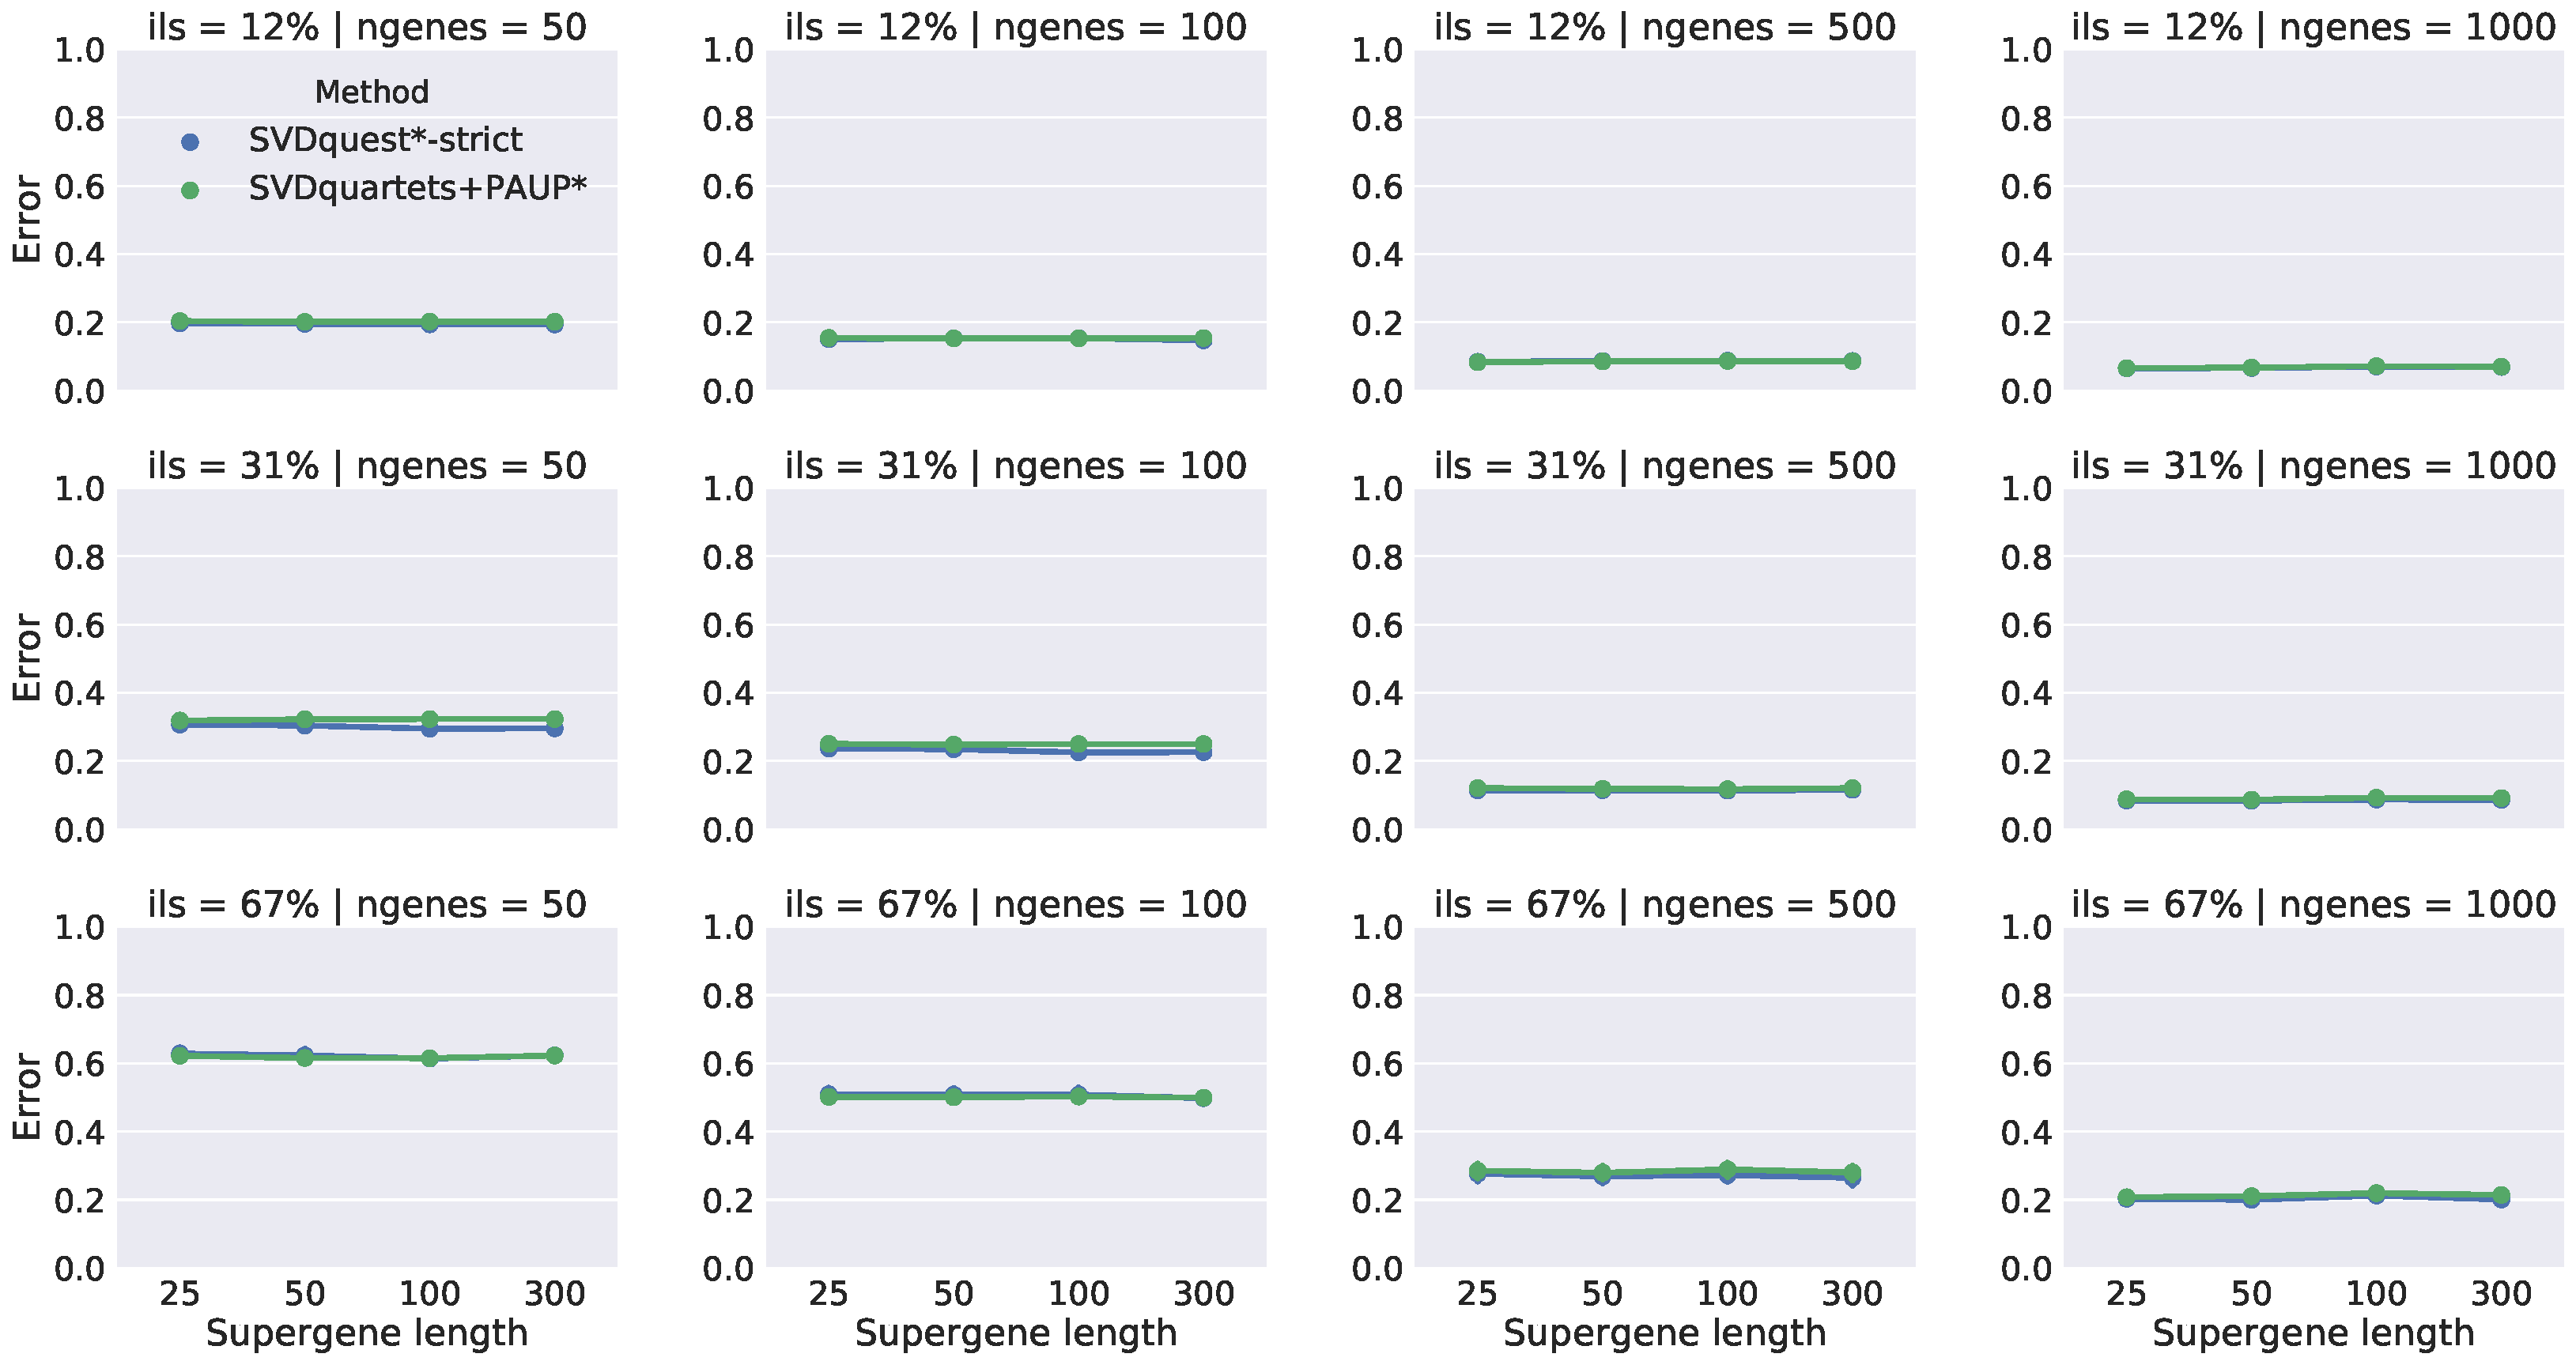
\includegraphics[width=\textwidth]{svdquest-figs/binned_rfdists_paup.pdf}
  \caption[Species tree error rates of SVDquest*-strict and SVDquartets+PAUP* on 50-taxon supergene datasets]{Species tree error rates (maximum is 1.0) of SVDquest*-strict and SVDquartets+PAUP* on 50-taxon simulated data using 
    supergenes (concatenations of c-genes), averaged over 40-50
    replicates per model condition (i.e. a specific combination of ILS level, number of genes, and sequence length). Error bars represent standard error of the mean. The c-genes are 25 sites long, and multiple loci were
    concatenated to form supergenes. Thus, the 
    25-site genes have sites coming from one locus, the 50-site genes have
    sites coming from two loci, and the 100-site genes have sites coming
    from four loci. Each data point in a particular subfigure represents
    an analysis on the same number of sites.
  }
  %\label{binned_50}
  \label{fig:s9}
\end{figure}

\clearpage

\begin{figure}
  \centering
  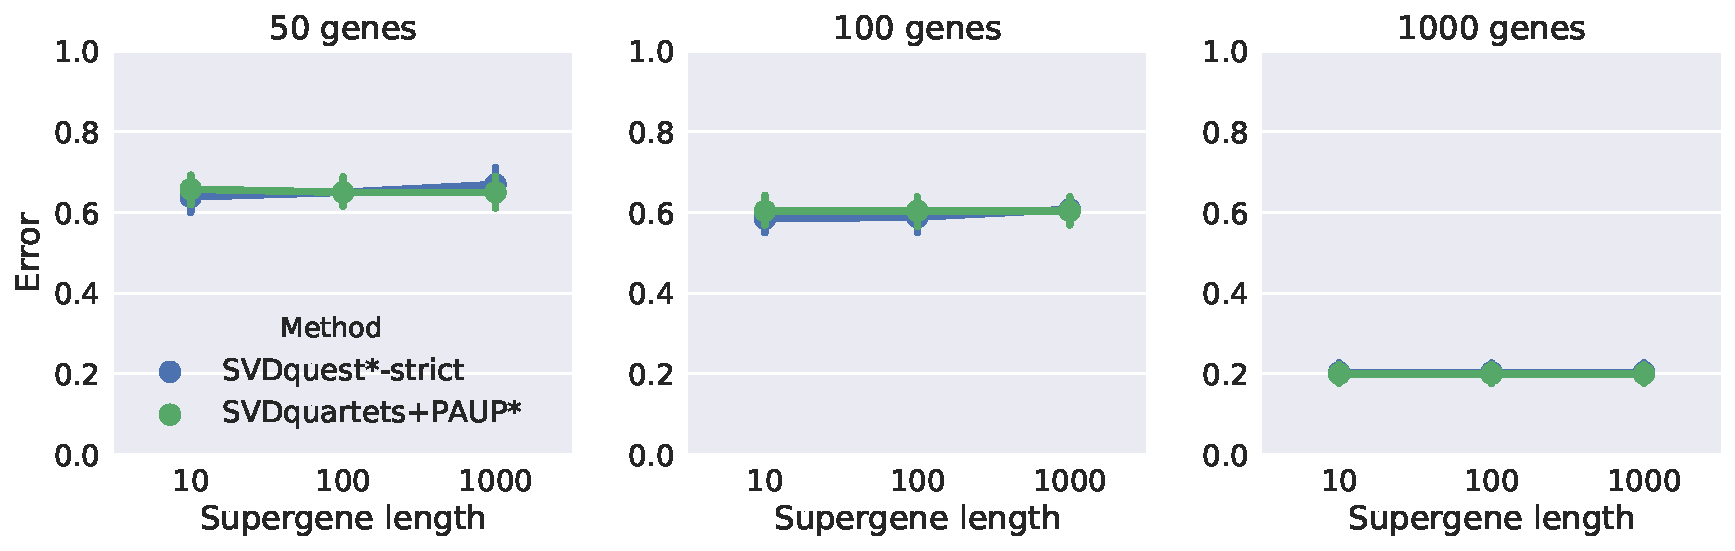
\includegraphics[width=\textwidth]{svdquest-figs/binned_rfdists_paup_15tax.pdf}
  \caption[Species tree error rates for SVDquest*-strict and SVDquartets+PAUP* on 15-taxon supergene datasets]{Species tree error rates (maximum is 1.0) on 15-taxon (AD 82\%) simulated data using 
    supergenes (concatenations of c-genes), averaged over 10
    replicates per model condition (i.e. a specific combination of number of genes and sequence length). Error bars represent standard error of the mean. The c-genes in this experiment are 10 sites long, and multiple loci were
    concatenated to form supergenes. Thus, the 
    10-site genes have sites coming from one locus, the 100-site genes have
    sites coming from 10 loci, and the 1000-site genes have sites coming
    from 100 loci. Each data point in a particular subfigure represents
    an analysis on the same number of sites.
  } %\label{binned_15}
  \label{fig:s10}
\end{figure}



\begin{figure}
  \centering
  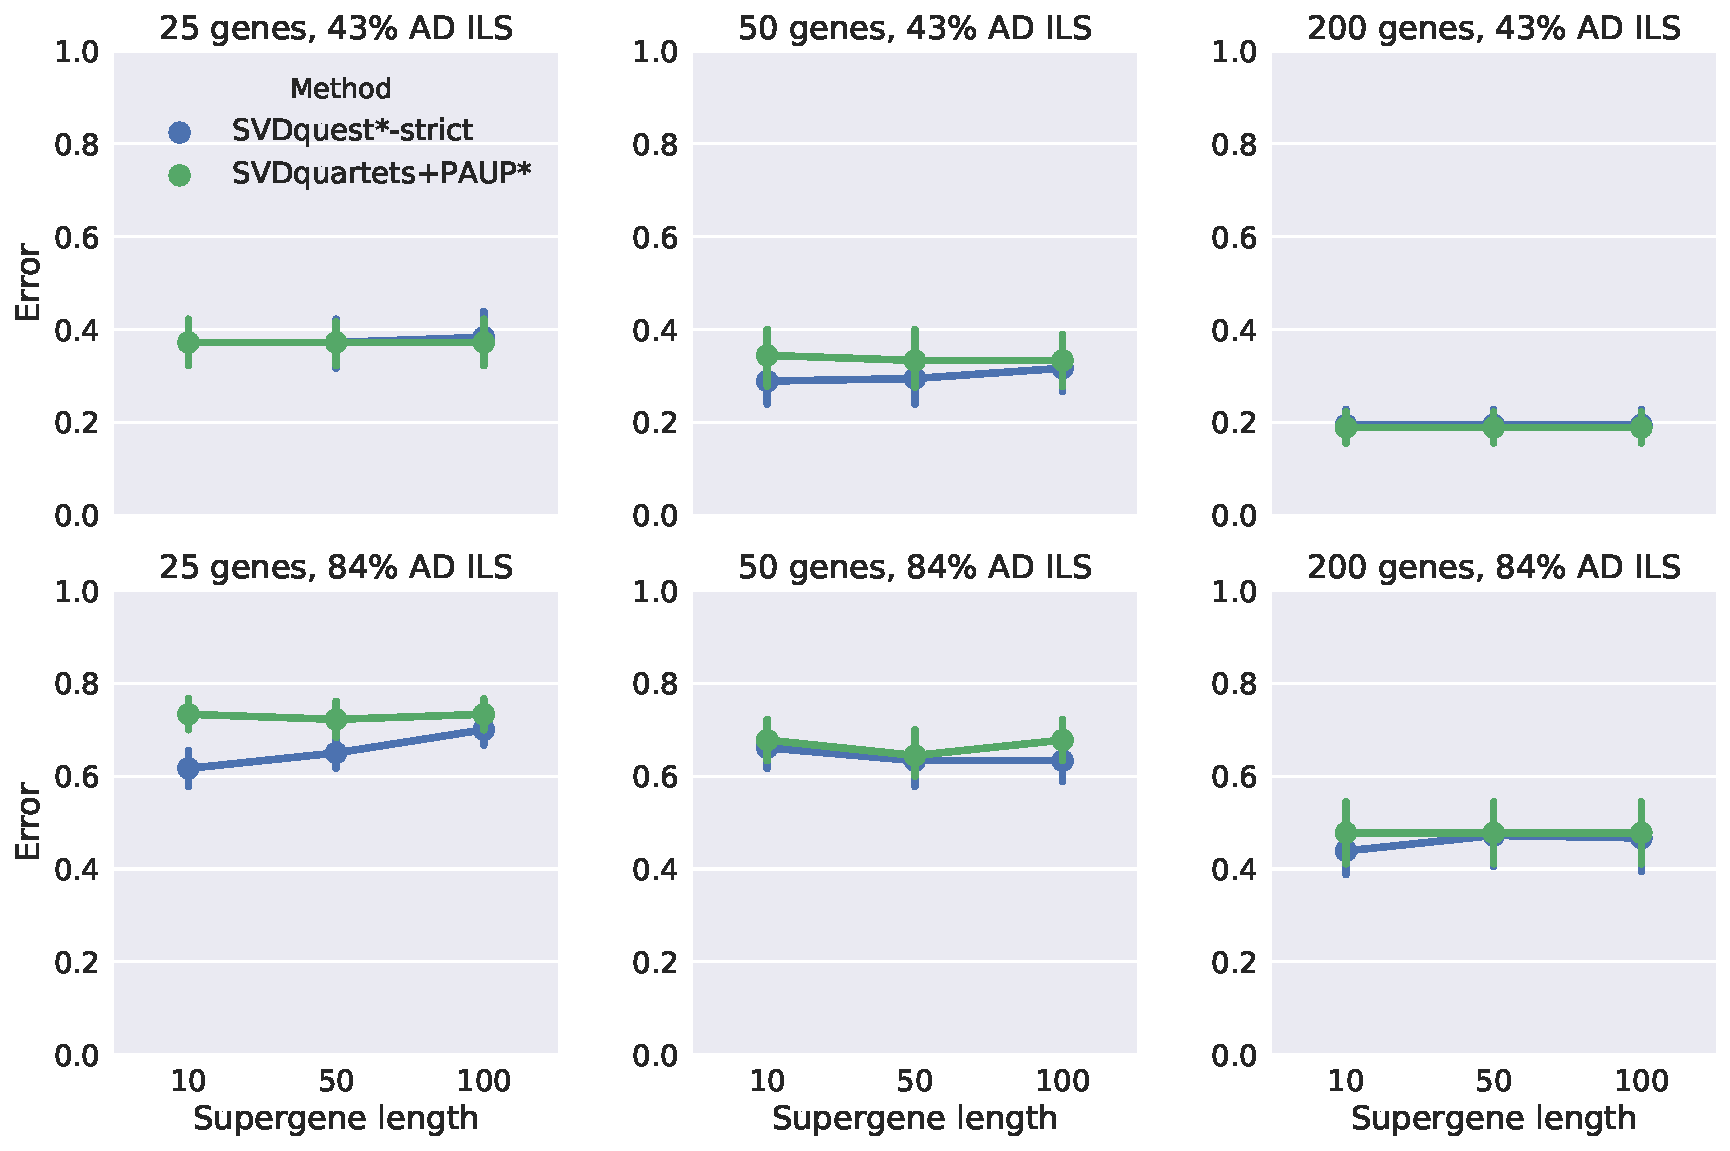
\includegraphics[width=\textwidth]{svdquest-figs/binned_rfdists_paup_10tax.pdf}
  \caption[Species tree error rates of SVDquest*-strict and SVDquartets+PAUP* on 10-taxon supergene datasets]{Species tree error rates (maximum is 1.0) on 10-taxon simulated data using 
    supergenes (concatenations of c-genes), averaged over 10
    replicates per model condition (i.e. a specific combination of ILS level, number of genes, and sequence length). Error bars represent standard error of the mean. The c-genes in this experiment are 10 sites long, and multiple loci were
    concatenated to form supergenes. Thus, the 
    10-site genes have sites coming from one locus, the 100-site genes have
    sites coming from 10 loci, and the 1000-site genes have sites coming
    from 100 loci. Each data point in a particular subfigure represents
    an analysis on the same number of sites.
  } %\label{binned_15}
  \label{fig:s11}
\end{figure}





\begin{figure}
  \centering
  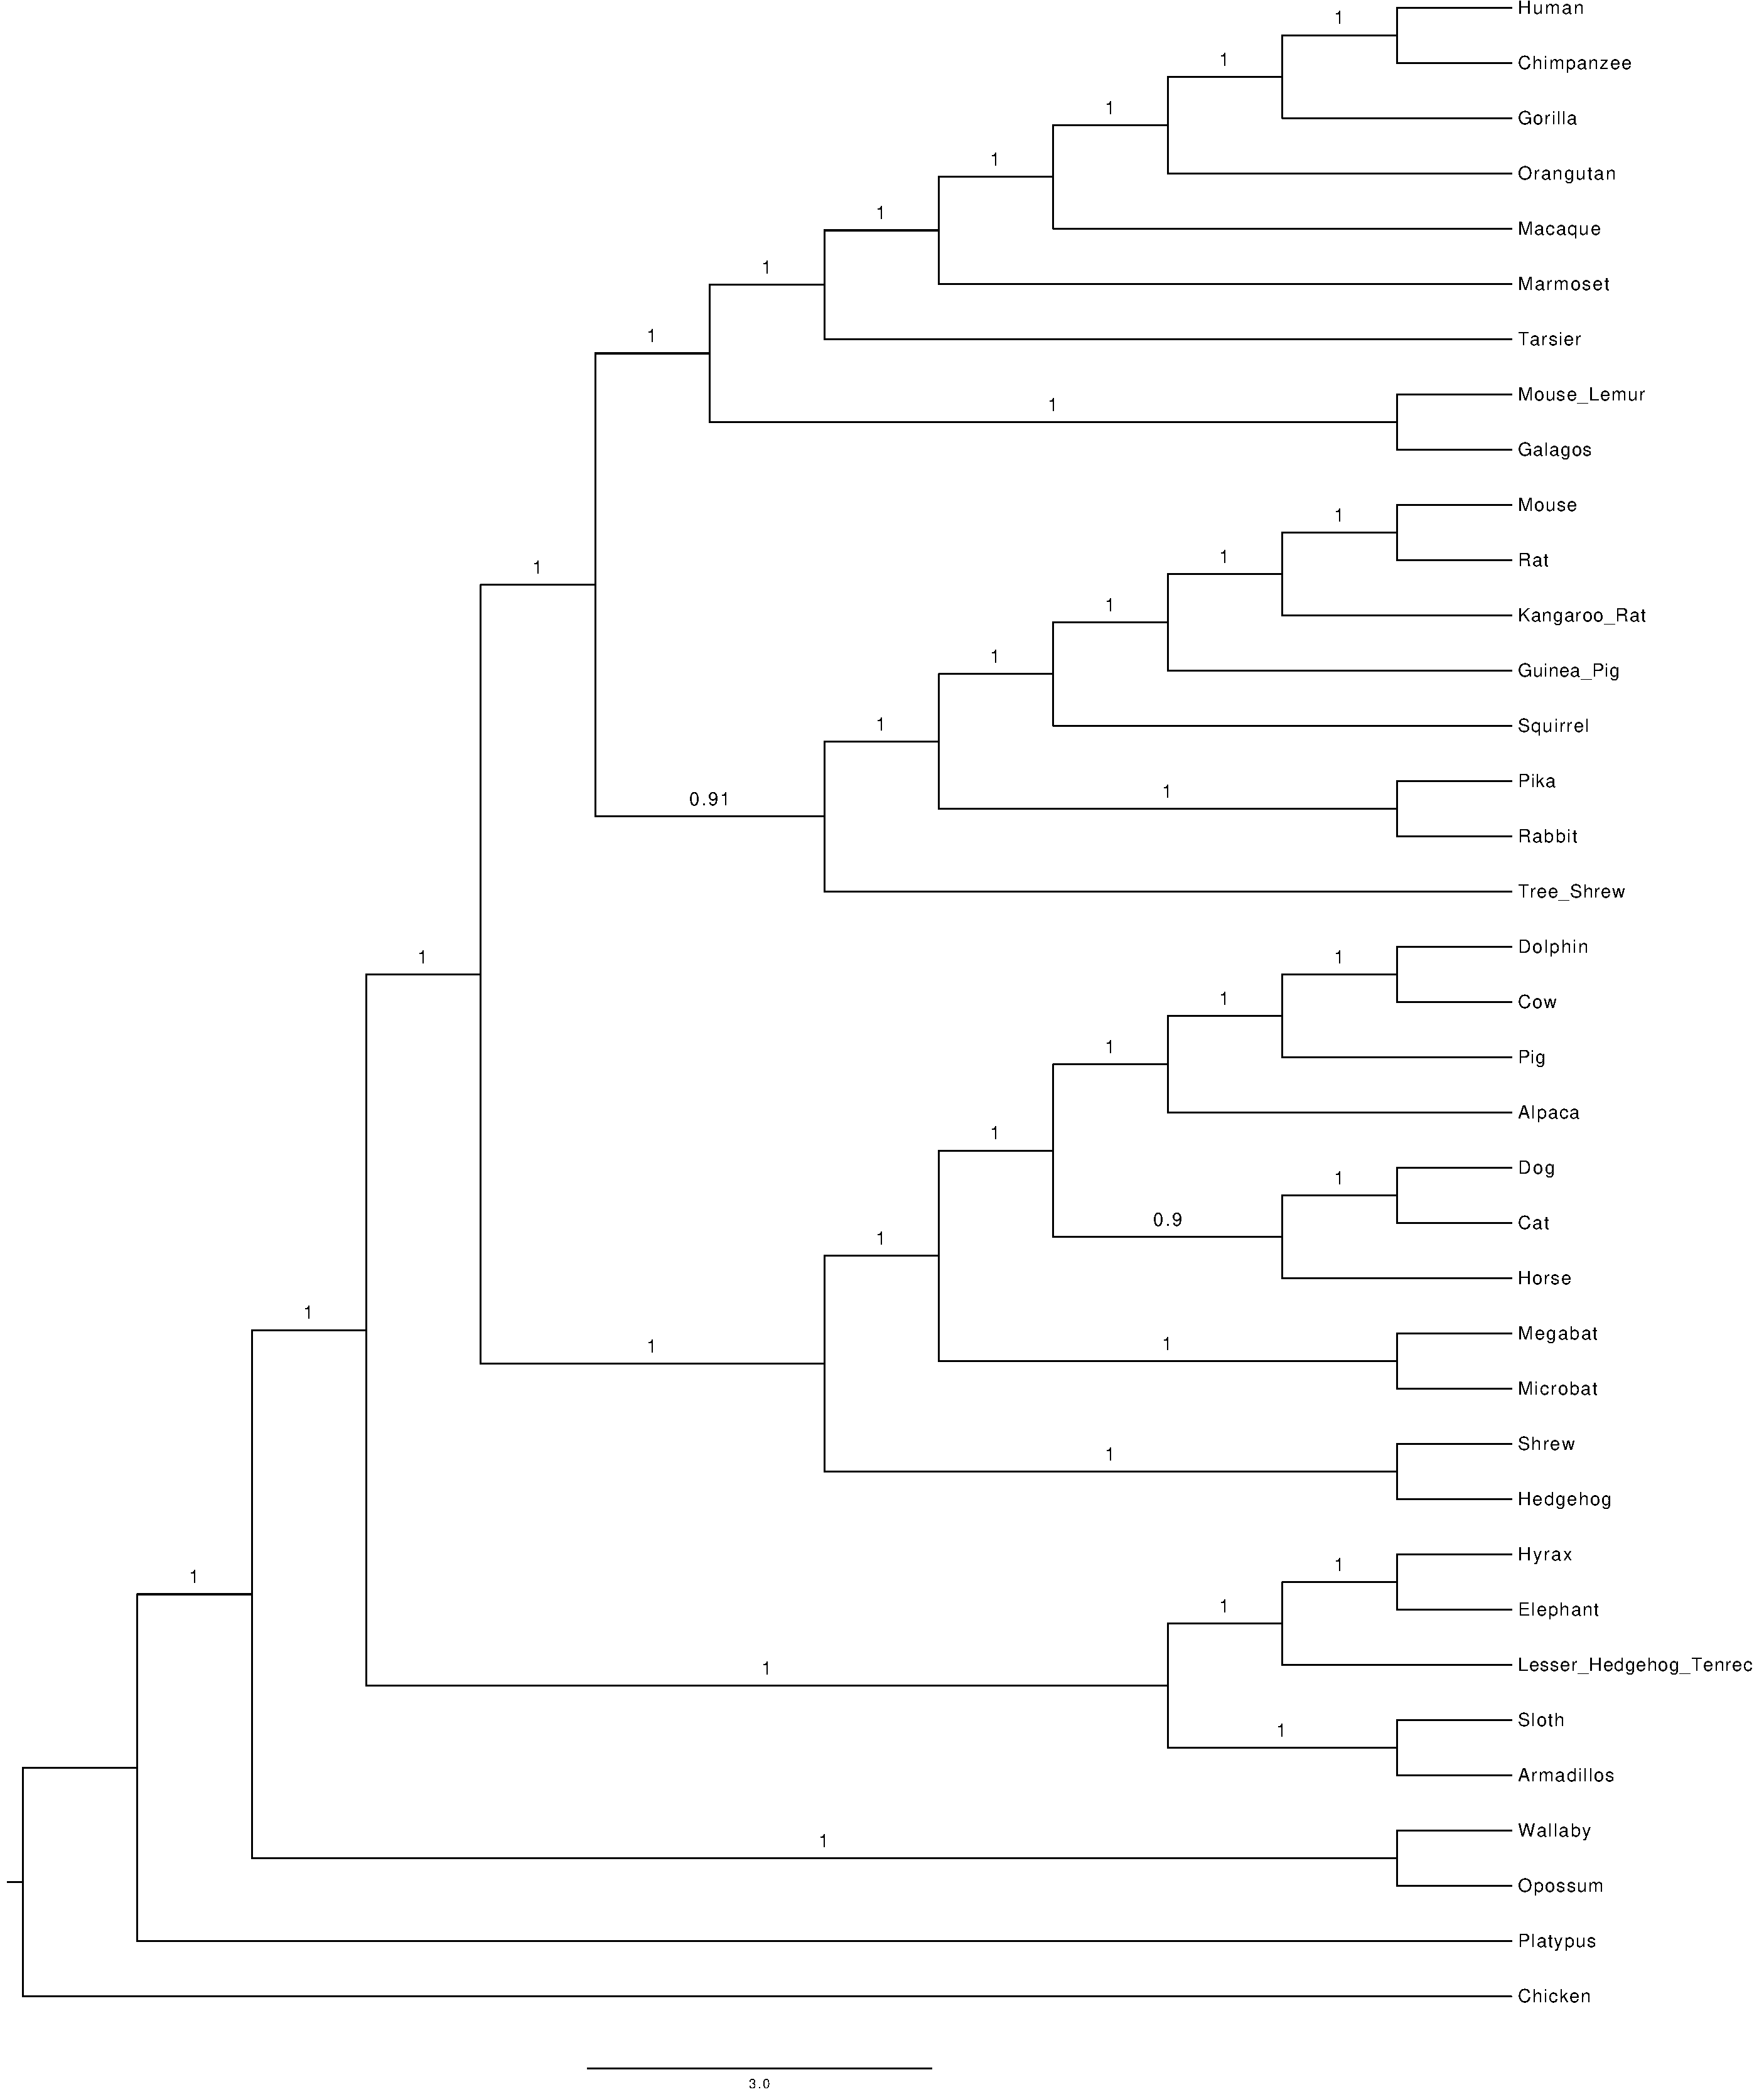
\includegraphics[width=\textwidth]{svdquest-figs/mammalian_astral_ann.pdf}
  \caption[Mammalian species trees computed using ASTRAL and ASTRID, with ASTRAL's local branch support]{Mammalian ASTRAL/ASTRID tree with branch support calculated using ASTRAL's local posterior support technique.}
%  \label{fig:mammalian-svdquestplus}
\label{fig:s12}
\end{figure}

\clearpage

\subsection{Cases where SVDquartets failed to return any quartet trees}
\label{svdquartets-failure}
On several model conditions, SVDquartets+PAUP* and SVDquest failed to return a tree; a review of these model conditions shows that SVDquartets returned the error message:
``No informative quartets were found in SVDQuartets analysis.''
Analysis of these datasets showed that each one had a very small number of parsimony-informative sites. The failing dataset with the most parsimony-informative sites had 13, and no dataset had more than one site exhibiting all four states.
See https://doi.org/10.6084/m9.figshare.5946736 for some of these datasets.
